%   %%%%%%%%%%%%%%%%%%%%%%%%%%%%%%
%   \chapter{Intro} 
%   
\seciton{Topological knots}

Let $M$ be a manifold (we will assume $\dim M \ge 3$, since $2d$ and $1d$ is of
little interest), then an immersion $K \subset M$ of $S^1$, is called a
\wddef{topological knot}.  
\todo{Move this to a section on topological knots}
In the study of topological knots, one are interested in whether two knots are
equivalent. That is whether one knot can be turned into the another,
through a continues transformation. More precisely, 

\begin{defn}
Let $K$ and $K'$ be topological knots. An \wddef{isotopy} from $K$ to $K'$ is
map
\[ H : [0,1] \times S^1 \to M, \]
such $H(0,s^1) = K$, $h(1,S^1) = K'$ and for each $t\in [0,1]$, $H(t, S^1)$ is a
topological knot. (That is $H$ is a path from $K$ to $K'$ in the space of
topological knots in $M$. ) If such a map exists we say $K$ and $K$ are
\wddef{isotopic}.
\end{defn}

If $M = \R^3$, it is interesting to study the projections onto an embedded plane
$\R^2$. For almost all planes this projection will be \wddef{regular}, that is
injective except at a finite number of points.

\begin{lemma}
Considering the projection of an isotopy $H$ from $K$ to $K'$. Then $H$ consist
of continues deformations through regular knots as well as a finite number of so
called Reidemeister moves. There are three such Reidemeister moves, see figure
\pref{reid_moves_top}.
\end{lemma}


\begin{figure}
\centering
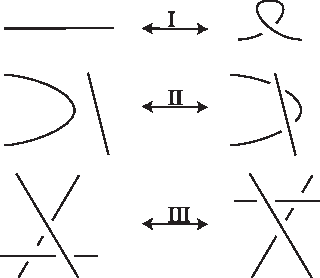
\includegraphics[width=.4\textwidth]{figs/reid_moves_top.pdf}
\caption{Topological Reidemeister moves}
\label{fig:reid_move_top}
\end{figure}
 %%% TODO

    %%%%%%%%%%%%%%%%%%%%%%%%%%%%%%
    \chapter{Legendrian Knots}
 
    \section{Contact Geometry}
    

\subsection{Definition}

A \wddef{contact structure} on an oriented 3-manifold $M$ is a certain kind of
plane filed over $M$. More precisely it is a rank 2 sub-bundle $\xi \subset TM$,
given locally by the kernel of a one-form $\alpha$ (ie. for all $x\in M$,
$\exists U \subset M$, such that $\xi_x = \ker(\alpha_x)$ for all $x\in U$)
satisfying 
\begin{equation} 
\label{eq:alpha_non_zero}
\alpha \wedge \d \alpha \ne 0. \quad \text{(ie. everywhere non-zero.)}
\end{equation}

We will also require that $\alpha \wedge \d \alpha$ agrees with the orientation
orientation of $M$.
Intuitively condition \pref{eq:alpha_non_zero}, require the planes to be
twisting, see figure \pref{fig:stand_contact}. Because of this twisting, there
can not be a surface in $S \subset M$, such that $\xi|S = TS$. 
A \wddef{contact manifold} is a pair $(M,\xi)$, where $M$ is an oriented
3-manifold and $\xi$ is a contact structure on $M$.

\begin{figure}
\centering
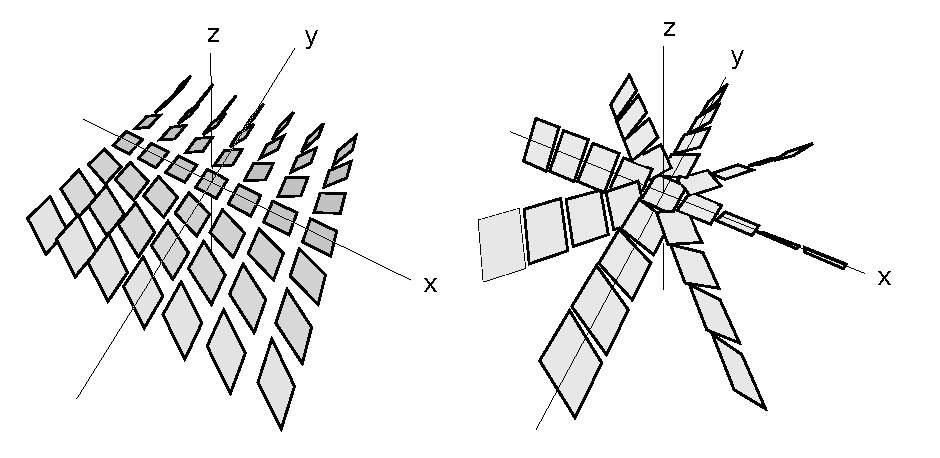
\includegraphics[width=.4\textwidth]{figs/stand_contact.pdf}
\caption{Contact structure $\xi_{std}$ (left) and $\xi_{sym}$ (right). }
\label{fig:stand_contact}
\end{figure}

\subsection{Examples}

\begin{exmp}
Consider $M = \R^3$, with Cartesian coordinates $(x,y,z)$. Let $\alpha = \d z -
y \d x$, then $\alpha \wedge \d \alpha = \d x \wedge \d y \wedge \d z \ne 0$.
Define 
\[ \xi_{std} := \ker{\alpha} = \spann\qty{ \dd{y}, \dd{x} + y \dd{z} }. \]
$\xi_{std}$ is called the standard contact structure on $\R^3$. See fig
\pref{fig:stand_contact}.
\end{exmp} 
There are a couple key features of this plane filed. 
Note that restricted to a plane parallel with the $xz$-plane all the planes are
parallel, or sad in a different way the pane filed is invariant under
translations orthogonal to the $y$ direction. In particular the planes along the
$xz$-plane are all horizontal, that is parallel with the $xy$-plane. On the
other hand, when moving along the $y$-axis the planes twist in a left hand
manner. Twisting a total of $90^\circ$ going from the origin "to infinity" in
the $y$-direction. 

\begin{exmp}
Again let $M = \R^3$ and let $\alpha = \d z + x\d y - y \d x$ ( or $\alpha = \d
z + r^2 \d \theta$ in cylindrical coordinates.) Then $\alpha \wedge \d \alpha =
2 \d x \wedge \d y \wedge \d z \ne 0$, so $\alpha$ defines a contact structure.
Define 
\[  \xi_{sym} := \ker\alpha = \spann\qty{ \dd{r}, \dd \theta - r^2 \dd{z} }. \]
This is the symmetric version of $\xi_{std}$.
\end{exmp}


%  
% = \spann{ (\dd x)^2 +  }

Here the planes are invariant under vertical translations (along the $z$-axis)
and rotation about the $z$-axis. 

\begin{defn}
Let $M$ and $N$, be two oriented 3-manifolds and suppose $\xi_M$ and $\xi_N$ are
are contact structures on $M$ and $N$ respectively. 
A diffeomorphism $f: M \to N$ is called a \wddef{contactomorphism}, if $f_*$ maps
$\xi_M$ to $\xi_N$. 

If such a contactomorphism exist $\xi_M$ and $\xi_N$ are sad to be
\wddef{contactomorphic}.
\end{defn}


The contact structures $\xi_{std}$ and $\xi_{sym}$ are contactomorphic, so in
a way they are the same structure. 
%
%Let $f(x,y,z) = (x, y, z - x^2y )$
%
% Df = 
%    1  0 0
%    0  1 0
% -2xy -x^2 1
%
% $ f^* \alpha (dx, dy, dz) = \alpha \circ f_* (  )
%
Also suppose we defined $\xi_{std}$ with
the opposite sign (ie. $\alpha = \d z + y\d x$), then the planes would instead
twist in a right handed manner, when moving in the $y$ direction. Then this
structure would be contactomorphic to $\xi_{std}$, by the diffeomorphism mapping
$y$ to $-y$.

\begin{exmp}
Let $M=\R^3$ and $\alpha = \cos r \d z + r \sin r \d \theta$ and define the
contact structure $\xi_{ot} = \ker \alpha$. See fig \pref{fig:overtwisted}
\end{exmp}

\begin{figure}
\centering
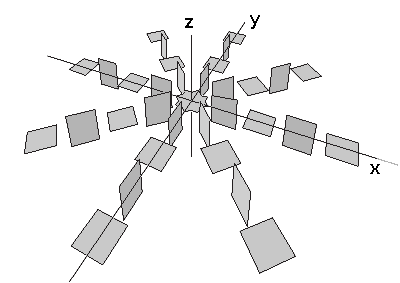
\includegraphics[width=.4\textwidth]{figs/overtwisted.pdf}
\caption{The overtwisted contact structure $\xi_{ot}$.}
\label{fig:overtwisted}
\end{figure}

Note how this structure in a way is very similar to $\xi_{sym}$, except that
when moving along a ray perpendicular to the $z$-axis, the twisting is much
quicker. So in instead of rotating a total of $90^\circ$ when going to infinity,
the planes are already twisted $90^\circ$ when getting to a radius of $\pi/2$ and
rotates an infinite number of times when going to infinity.

\begin{defn}
Suppose $\xi$ defines a contact structure on $M$. Then, we say $\xi$ is
\wddef{overtwisted}, if there exist an immersion $u : D(0,1) \to M$, where
$D(0,1) = \{ (x,y) \in \R^2 \q| x^2+y^2 \le 1 \}$ is the unit disk, such that
\[ \xi|_{\partial D} = TD|_{\partial D}. \]
(ie. $\xi$ is tangent to $D$ along the border of $D$.) Such a disk immersion is
called an \wddef{overtwisted disk}.

If $\xi$ is not overtwisted we say $\xi$ is \wddef{tight}.
\end{defn}

Clearly $\xi_{ot}$ is overtwisted since $D = \{ (r,\theta, z) \q| z = 0, 0 \le
r \le 1\}$ is an overtwisted disk. On the other hand $\xi_{std}$ and $\xi_{sym}$
are tight. It turns out that tight contact structures are more interesting then
the overtwisted ones, see \cite{Eliashberg1989}. In this paper we will mainly
concentrate on $(\R^3, \xi_{std})$. However, we will mention one other example.   

\begin{exmp}
Let $M=S^3$ considered as the unit sphere in $\R^4$ (with Cartesian coordinates
$(x_1,y_1,x_2,y_2)$), and let 
\[ \alpha = i^*( x_1 \d y_1 - y_1 \d x_1 + x_2 \d y_2 - y_2 \d x_2 ), \]
where $i: S^3 \R^4$ is the inclusion map. One may check that $\alpha \wedge \d
\alpha \ne 0$, and define $\xi = \ker \alpha$.
\end{exmp}

By removing one point $p$ from $S^3$, the contact structure $\xi$ on $S^3 \setminus
\{p\}$ is
contactomorphic to $\xi_{sym}$ (and thus $\xi_{std}$) on $\R^3$. 

In fact, if we associate $\R^4$ with $\C^2$, we can construct this contact
structure from the complex structure on $C^2$. Let $J$ denote complex
multiplication in $\C^2$, ie. $J x_i = y_i$ and $J y_i = x_i$ for $i=1,2$. This
complex structure includes a complex structure on the tangent space $J
\dd{x_i} = \dd{y_i}$ and $J\dd{y_i} = \dd{x}$.

\begin{clame}
Then $\xi$ is the complex tangents of $S^3$. ie.
\[  \xi = TS^3 \cap J (TS^3), \]
that is the tangent space closed under complex multiplication. 
\end{clame}

\begin{proof}
Let $f:R^4 \to R^4$, defined by $f(x_1,y_1,x_2,y_2) = x_1^2+y_1^2+x_2^2+y_2^2$,
then $S^3 = f^{-1}(1)$. Then the tangent space of $S^3$ at $(x_1,y_1,x_2,y_2)$
\[ T_{(x_1,y_1,x_2,y_2)}S^3 = \ker{ \d f_{(x_1,y_1,x_2,y_2)} },   \]
and 
\[ J (T_{(x_1,y_1,x_2,y_2)}S^3) = \ker{ \d f_{(x_1,y_1,x_2,y_2)} \circ J}. \]
Since 
\[ \d f_{(x_1,y_1,x_2,y_2)} \circ J = 2 x_1 \d y_1 - 2 y_1 \d x_1 + 2 x_2 \d y_2 - 2 y_2 \d x_2 \]
So $\alpha = (\d f \circ J)|_S^3$, which proves the clime.
\end{proof}


% \subsection{Relation to simplistic geometry}


 
    \section{Legendrian Knots}
    
\subsection{Definition}

% \begin{defn}
% Let $(M,\xi)$ be a contact manifold. A \wddef{Legendrian knot} $L$ in $(M,\xi)$ is
% an embedding $\gamma: S^1 \to M$, such that $L = \gamma(S^1)$ and 
% \[ \left. \dif{\gamma}{t} \right|_{t'} \subset \xi_{\gamma(t')}. \] 
% \end{defn}

\begin{defn}
Let $(M,\xi)$ be a contact manifold. A \wddef{Legendrian knot} $L \subset M$ is
an embedding of $S^1$, such that 
\begin{equation}
\label{eq:l_knot_eq}
T_x L = \xi_x, \quad \forall x\in L. 
\end{equation}
\end{defn}

For the rest of this paper we will assume $(M,\xi) = (\R^3,\xi_{std})$. Most of
the discussions and result generalize to general contact manifolds. But for
simplicity we will stick with this particular case. This allows us to work in
terms of the projections onto the coordinate planes, which will simplify some of
the arguments significantly. In particular the proofs found in chapter
\pref{chap:proofs}, will naturally simplify to a combinatorial argument.

\subsection{Projections}

For this section it will convenient to have a parametrization for $L$. Let
\[ \gamma : S^1 \to L; \: t \mapsto (x(t), y(t),z(t)), \] 
be a $C^1$ (ones continuously differentiable) parametrization of $L$. Then we 
can be written equation \pref{eq:l_knot_eq},
\[ \gamma'(t) \subset \xi_{\gamma(t)}, \quad \forall t\in S^1, \] 
or equivalently, since $\xi = \xi_{std} = \ker{\d z - y\d x}$, 
\begin{equation}
\label{eq:std_l_knot_eq}
z'(t) - y(t) x'(t) = 0.
\end{equation}

\begin{defn}
\wddef{Front projection} is the map
\[ \Pi : \R^3 \to \R^2; \: (x,y,z) \mapsto (x,z), \]
\end{defn}

Let $\phi_\Pi = \Pi \circ \gamma$.  By equation \pref{eq:std_l_knot_eq}, $z'(t)
= y(t) x'(t)$, so if $x'(t) = 0$, $z'(t) = 0$. Therefore $\Pi(L)$ can not have
any vertical tangents \big(ie.  $\phi_\Pi'(t) \notin \spann\qty{\dd{z}}
\setminus\{0\}$ for all $t$. \big) Also $(\phi_\Pi)'(0) = 0$, whenever $x'(t) =
0$, so $\phi_\Pi$ is on not an immersion. On the other hand, away from $x'(t) =
0$ (ie. $t \in I \setminus x'^{-1}(0)$), $\phi_\Pi$ is an immersion.  If $x'(t)
\ne 0$, by equation \pref{eq:std_l_knot_eq}, we may recover $y(t)$ from the
projection
\[ y(t) = \frac{z'(t)}{x'(t)}. \]

A point in $\Pi(L)$ where $x'(t) = 0$ we will call a "cusp point". Here the
tangent of $L$ is parallel with the $y$-axis. See figure \pref{fig:cusp_point}.

\begin{figure}
\centering
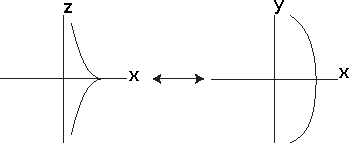
\includegraphics[width=.4\textwidth]{figs/cusp_point.pdf}
\caption{Front and Lagrangian projection of a part of a Legendrian knot where
$x'(t) = 0$ (ie. a cusp point, in the front projection.)}
\label{fig:cusp_point}
\end{figure}

\begin{lemma}
A diagram $D \subset \R^2$, is the Front projection of a Legendrian knot
if and only if:
\begin{enumerate}
\item
There are no vertical tangents.
\item 
$D$ is an immersion away from a finite collection of cusp, points.
\item 
At each crossing the slope of the overcrossing is less then the slope of the
undercrossing.
\end{enumerate}
\end{lemma}

\begin{exmp}
In figure \pref{fig:front_knots} we can see the front projection of a Legendrian
realization of the unkont, left and right handed trefoil knot and the figure of
eight knot.
\end{exmp}

\begin{figure}[h]
\centering
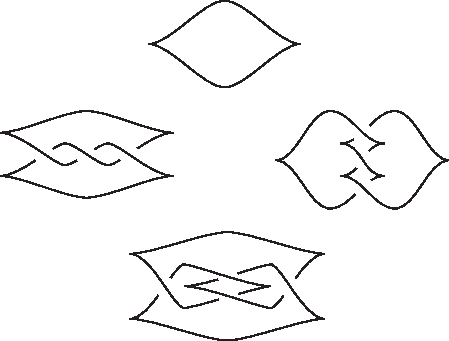
\includegraphics[width=.4\textwidth]{figs/front_knots.pdf}
\caption{Front projection of Legendrian realization of the unknot, left and
right handed trefoil knots and the figure of eight knot.}
\label{fig:front_knots}
\end{figure}

\begin{defn}
The \wddef{Lagrangian projection} of $L$ is the map
\[ \pi : \R^3 \to \R^2; \: (x,y,z) \to (x, y), \]
\end{defn}

Let $\phi_\pi = \pi \circ \gamma$. In contrast with the front projection,
$\phi_\Pi$ is always an immersion, since by equation \pref{eq:std_l_knot_eq}, if
$x'(t) = 0$ also $z'(t) = 0$ and thus $y'(t) \ne 0$, as $\phi$ is an immersion.

By integrating equation \pref{eq:std_l_knot_eq}, we have 
\[ z(t) = z_0 + \int_0^t y(t') x'(t') \d t',  \]
( Here we consider $t \in [0,2\pi)$ ) so we may recover the z-component of $L$ from the projection up to an overall
factor $z_0$. Note that for $L$ to be closed we require $z(2\pi) = z_0$, so 
\begin{equation}
\label{eq:lagrangian_pr_eq}
\int_S^1 y(t) x'(t) \d t = 0.
\end{equation}

\begin{lemma}
A diagram $D \in \R^2$ is the Lagrangian projection of a Legendrian knot if and
only if
\begin{enumerate}
\item $D$ is an immersion.
\item 
$\int_S^1 y(t) x'(t) \d t = 0$, where $(x,y): S^1 \to \R^2$ is a
parameterization of $D$.
\item 
$\int_{t_1}^{t_2} y(t) x'(t) \d t = 0$, if $(x(t_1),y(t_1)) = (x(t_2),y(t_2))$.
\end{enumerate}
\end{lemma}

This projection will be the more interesting for us. Though the constraints (ie.
\pref{eq:lagrangian_pr_eq}), given by the Legendrian condition \pref{eq:l_knot_eq}, is a little harder to work with. 

\section{Reidemeister moves}

Like in the case of topological knots, there are also Legendrian Reidemeier
moves for these projections, see figure \pref{fig:reid_move_top}

\begin{figure}
\begin{minipage}[c]{.5\textwidth}
\centering
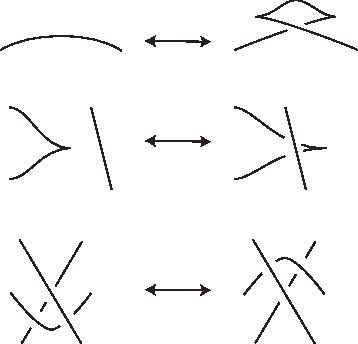
\includegraphics[width=.8\textwidth]{figs/reid_moves_front.pdf}
\caption{Legendrian Reidemeister moves in front projection.}
\label{fig:reid_move_top}
\end{minipage}
\begin{minipage}[c]{.5\textwidth}
\centering
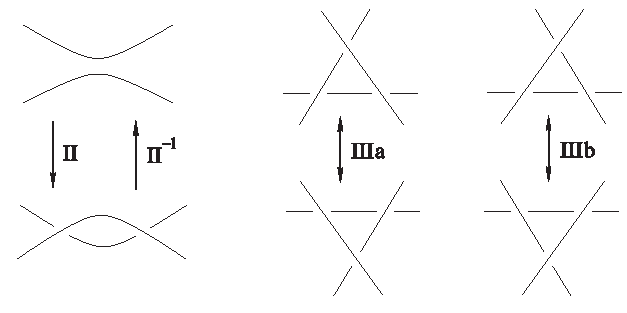
\includegraphics[width=.8\textwidth]{figs/reid_moves.pdf}
\caption{Legendrian Reidemeister moves in Lagrangian projection.}
\label{fig:reid_move_top}
\end{minipage}
\end{figure}

% \subsection{The existence of Legendrian knots of any top know}

    
    \section{Classical Invariants}
    

\begin{defn}
Let $\gamma: [0,1] \to \R^2$ be a smooth curve. The \wddef{gausian map of
$\gamma$} $g: [0,1] \to S^1 \subset \R^2$ is given by
\[ g(t) = \frac{\gamma'(t)}{\|\gamma'(t)\|}. \] 
Where $S^1 \subset \R^2$ is thought of as the unit circle.

Consider the quationt map $q: \R \to \R/\Z = S^1$. There is a unique
(up to translation by $\Z$) lift (by $q$) of $g$, $\tilde{g}$, ie. a map
$\tilde{g}:[0,1]\to \R$ such that $g = q \circ \tilde{g}$. 

rotation number of $r(\gamma) = g(1) - g(0) \in \R$.

Then the \wddef{rotation number of $\gamma$} is $r(\gamma) =
\tilde{g}(1) - \tilde{g}(0)$.
\end{defn}

Note that, if the path is closed, $r(\gamma) \in \Z$. Also the rotation number
invariant under reparameterization, so we may write $r(\im(\gamma))$.
(In particualt we will write $r(L) \in \Z$, for the rotation number of $L$ )

 %%% TODO
 
    %%%%%%%%%%%%%%%%%%%%%%%%%%%%%%
    \chapter{The associated \Ainf algebra}
    \label{chap:assic_a_alg}

    \section{\Ainf-algebras}
    
\subsection{Definition}

\begin{defn}
Let $k$ be a field and $\Gamma = \Z/c\Z$ be a cyclic group, for some
$c\in \Z$. An \wddef{\Ainf-algebra over $k$} is a $\Gamma$-graded 
vector space
\[ A = \bigoplus_{p\in\Gamma} A^p  \]
endowed with a family of graded $k$-linear maps
\[ m_n: A^{\otimes n} \to A, n \ge 0, \]
of degree $2-n$ (mod $c$) satisfying the \Ainf relations:

\begin{equation}
\label{eq:Ainf_rels}
\sum_{r+s+t = n} (-1)^{r+st} m_u(\I^{\otimes r} \otimes m_s \otimes \I^{\otimes t}) = 0.
\end{equation}
Where the sum runs over all $r,s,t \ge 0$, such that $r+s+t=n$ and $u = r+1+t$. 
\end{defn}

\subsubsection{Remark:}
Often this definition is known as a \wddef{curved} \Ainf-algebra, where $m_0$ is the \wddef{curvature} of $A$. If $m_0 = 0$ we say $A$ is \wddef{uncurved}.
If $A$ is uncurved, the first \Ainf relation
(ie. $n=1$), demands that $m_1 \circ m_1 = 0$ and we may define the \wddef{cohomology}
$H^*(A,m) = \ker(m_1)/\im(m_1)$, a graded $k$-vector space.
The second \Ainf relation is
\[ m_2(m_2 \otimes \I + \I \otimes m_2), \]
so $m_2$ defines a product on the \wddef{cohomology}, which by the third relation if associative.

In this notes we will, by an \Ainf-algebra, refer to the more general
case of a curved \Ainf-algebra.

\subsubsection{Notation}
Let
\[ TA := \bigoplus_{n\in\Z} A^{\otimes n} \]
denote the tensor-algebra generated by $A$, with the canonical product 
\[ w: TA\otimes TA \to TA; \: (v,w) \mapsto v\otimes w. \]
Then the family $m_n: A^{\otimes n} \to A$ may be writen as a single map $m: TA \to
A$. Throughout this paper we will write an \Ainf-algebra as a pair $(A,m)$, where 
$m: TA \to A$.

If $a \in A$, them we will write $|a| \in \Gamma$ to denote the degree of $a$.

% Note that if we have $a_1,...,a_n \in A$, the relation above reads 
% \begin{equation}
% \label{eq:rel_on_a}
% \xi_n(a_1, ... a_n) =
% \sum_{r+s+t = n} m_u(a_1,..., a_r, m_s( a_{r+1}, ..., a_{r+s} ), a_{r+s+1},
% ..., a_n) = 0. 
% \end{equation}

\begin{defn}
An \Ainf-algebra $(A,m)$ is \wddef{finite} if there exists $N$ such that
\[ m_n = 0, \q{\text{for all}} n\ge N.  \]
\end{defn}

\subsection{Morphisms}

\begin{defn}
Let $(A,m^A)$ and $(B,m^b)$ be \Ainf-algebras. An \wddef{\Ainf-homomorphism} 
$f:A \ato B$ is a family of graded $k$-linear maps
\[ f_n : A^{\otimes n} \to B, n\ge 0 \]
of degree $1-n$ such that

\begin{equation}
\label{eq:ainf_morph_rel}
\sum (-1)^{r+st} f_u(\I^{\otimes r} \otimes m^A_s \otimes \I^{\otimes t}) 
= \sum (-1)^s m^B_r (f_{i_1} \otimes f_{i_2} \otimes ... \otimes
f_{i_r}),
\end{equation}
where the first sum runs over all decompositions $n = r+s+t$, like in
(\ref{eq:Ainf_rels}), and the second sum runs over all $1 \le r \le n$ and all
decompositions $n = i_1 + ... + i_r$. The sign on the right hand side is given
by
\[s = \sum_{j=1}^{r-1} (r-j)(i_j-1).  \]
\end{defn}

$f_0$ is called the \wddef{curvature} of $f$ and if $f_0 = 0$ we say $f$ is
\wddef{uncurved}.
If $(A,m^A)$, $(B,m^B)$ and $f$ are all uncurved, then the first \Ainf-relation is 
\[ f_1 \circ m^A_1 = m^B_1 \circ f_1. \]
So $f_1$ induces a linear map between the cohomologies
\[ f^* : H^*(A, m^A) \to H^*(B,m^B). \]
Note that the further conditions demands that the induced linear map, also
conserves the other algebraic structure on the cohomology. In particular the
second relation ($n=2$), implies that 
\[ f^* \circ m_2^* = m_2(f^* \otimes f^*), \]
where $m_2^*$ is the product induced by $m_2$. So the linear map is in
particular a homomorphism of algebras.

\begin{exmp}
If $(A, m)$ is an \Ainf-algebra, the identity $\id^A : A \ato A$ given by
\[ \id^A_i = \pwf{ \id &\tif i = 1 \\ 0 &\tif i \ne 1, } \]
is an \Ainf-homomorphism.
\end{exmp}

\begin{defn}
If $(A,m^A)$ and $(B,m^B)$ are finite and $f:A \ato B$ is an \Ainf-homomorphism, we say $f$ is \wddef{finite} if there exists $N$, such that $f_n = 0$ for all $n > N$.

If $N = 1$ and $f_0 = 0$, we say $f$ is \wddef{strict}.
\end{defn}

\begin{defn}
\label{def:Ainf_comp}
The \wddef{composition} of two \Ainf-homomorphisms $f: B \ato C$ and $g: A \ato B$ is given
by
\begin{equation}
\label{eq:ainf_comp_rel}
(f \circ g)_n := \sum (-1)^s f_r \circ (g_{i_1} \otimes ... \otimes
g_{i_r}),
\end{equation}
where the sum and sign are the same as in the defining identity.
\end{defn}

\begin{lemma}
The composition $f \circ g: A \ato C$, defines a new \Ainf-homomorphism and if both
$f$ and $g$ are finite, so is 
\end{lemma}

\begin{proof}
Through a simple swap of sums it is relatively easy to show that $f\circ g$,
indeed satisfy (\ref{eq:ainf_morph_rel}). 

Suppose $N\in \N$, is such that $f_n = 0$ and $g_n = 0$ for all $n > N$, then if
$n > N^2$, either $r > N$ or at least one $i > N$. So $(f \circ g)_n = 0$.
\end{proof}

\begin{defn}
An \Ainf homomorphism $f: A\ato B$, is an \wddef{isomorphism} if there exists an 
\Ainf-homomorphism $g: B\ato A$, such that \[ g \circ f = \id^A \qq\tand f \circ g = \id^B. \]
\end{defn}

\begin{lemma}
\label{prop:Ainf_iso_induced}
Let $(A,m^A)$ and $(B,m^b)$ be uncurved \Ainf-algebras. If $f: A \ato B$ is
an \Ainf-isomorphism, then the induced linear map $f^*: H^*(A,m^A) \to
H^*(B,m^B)$ is also an isomorphism of graded vector spaces.
\end{lemma}


\todo{move}

\begin{lemma}
\label{lemma:Ainf_struct_from_pre_hom}
Let $(A,m)$ be an \Ainf-algera and $f : A \ato A$ an \Ainf-pre-homomorphism,
such that $f_1$ is an isomorphism. Then there exists a unique \Ainf-structure
$\tilde{m}$ such that $f$ is an \Ainf-homomorphism from $(A,m)$ to
$(A,\tilde{m})$.
\end{lemma}

\begin{proof}

\[ \tilde{m}_k (f_1(a_1),...,f_1(a_k)) = P(f_i, \tilde{m}_{\le k-1} \}, m_j).  \]

\end{proof}




\begin{proof}
By definition, $(f\circ g)_1 = f_1 \circ g_1$. So $(f \circ g)^* = f^* \circ
g^*$. Hence $f^* \circ g^* = \id_{H^*(A,m^A)}$ and $g^* \circ f^* =
\id_{H^*(B,m^B)}$ and thus $f^*$ is invertible. Since $f_1$ has degree $0$,
so does $f^*$.
\end{proof}

\subsection{Tame morphisms}
\begin{defn}
Let $(A,m^A)$ be an \Ainf-algebra, where $A = k\<{a_1,...,a_n}$. An \Ainf-automorphism $f: A \ato A$ is called
\wddef{elementary} if there exist $j \in \{1,...,n\}$ and $u: TA \to k$, such
that for all $m \in \N$
\[ u_m(...,a_j,...) = 0 \q\tand f_m(a_{i_1},...,a_{i_m}) = \id^A + a_j u(a_{i_1},...,a_{i_m}), 
\]
A finite composition of such \Ainf-automorphisms is called \wddef{tame automorphism}.
A \wddef{tame \Ainf-isomorphism} $f: A \ato B$ is the composition of a tame automorphisms and a strict isomorphisms. 
\end{defn}
\subsection{Stabilization}

\begin{defn}
Let $(A,m)$ be an \Ainf algebra. The \wddef{$i$-th stabilization} of $A$, is a
new \Ainf-algebra $\qty(S_i(A), m^{S_i(A)})$, where
\[ S_i(A) = A \oplus k\<{e_1, e_2}, \]
$|e_1| = i$, $|e_2| = i+1$, 
\[ m_1(e_1) = e_2, \quad m_1(e_2) = 0, \quad m_n(..., e_j, ...) = 0 \quad \forall n \ne 1 \]
and $m^{S_i(A)} (a_1,...,a_n) = m_n(a_1,...,a_n)$ for all $n\in \N$ and $a_1,...,a_n \in A$.
\end{defn}

\begin{defn}
Let $(A,m^A)$ and $(B,m^B)$ be \Ainf-algebras, then they are sad to have the same \wddef{stable type} if there exist 
$i_1,...,i_k,j_1,...,j_l \in \Z$ and a tame \Ainf-isomorphism
\[ f: S_{i_1} (...(S_{i_k} (A, m^A))...) \to S_{j_1} (...(S_{j_l} (B, m^B))...). \] 
\end{defn}

Let $\sigma: S_i(A) \ato A$ and $\tau : A \ato S_i(A)$, such that $\sigma_k
= \tau_k = 0$ for $k> 1$, and 
\[ \tau_1(a) = a, \sigma_1(a) = a, \q\tand \sigma_1(e_j) = 0, \]
for all $a \in A$ and $j = 1,2$. ie. $\tau$ is the inclusion of $A$ in
$S_i(A)$ and $\sigma$ is the projection of $S_i(A)$ onto $A$.


\todo{ This is not done !!! }


\begin{lemma}
\label{lemma:tau_id_homotopy}
There exists a graded linear map $h: TS_i(A) \to TS_i(A)$, such that 
\[ \tau + \id_{S_i(A)} = h \circ m^{S_i(A)} + m \circ h\]

$\tau \circ \sigma$ is homotopic to $\id_A'$ as \Ainf-hom. 
\end{lemma}






    
    \section{Constructing the \Ainf algebra} 
    \label{sect:a_inf_alg_const}
    
In this section we will to every Legendrian knot ( or more acuratly the
Legendrian projection ) assosiate a finite \Ainf-algebra. This contruction
directly corresonds to the Chekanov-Eliashberg DGA constricted in
(\cite{chekanov02}).

Let $L$ be a Legendrian knot in the standard contact structure on $\R^3$.

\subsection{The vector space}
\begin{defn}
$L$ is sad to be \wddef{generic} wrt. $\pi$, if the set of crossings in $\pi(L)$
is finite and consist of transversal double points. More precisely, if $c\in
\pi(L)$ is a crossing. Then $\pi^{-1} \cap L = \{ c^+, c^- \}$ and if $T^\pm$
is the tangent line of $L$ at $c^\pm$, then $\pi(T^+) \cap \pi(T^-) = \{c\}$.
\end{defn}

For the rest if this paper will assume $L$ is generic and let $Y = \pi(L)$. ( Note that, any Legendrian knot is $C^\infty$-close to a generic one,
ie. there exist a smooth one parameter family of Legendrian knots $\{L_\alpha
\}\alpha \in [0,1]$, such that $L = L_0$ and $L_\alpha$ is generic for $\alpha >
0$. ) 

\begin{defn}
Let $\Cc = \{ a_1, \dots, a_n\}$ denote the set of double points in $Y$ and
$A = \Z_2\left<\Cc\right>$, be the $\Z_2$-vector space generated by $\Cc$.
\end{defn}

This vector space will be the base space, for the \Ainf-algebra. The grading 
on the vector space will take values in the cyclic group $\Gamma = \Z / m(L) \Z$, 
where $m(L)$ is twice the rotation number of $L$. To define the grading on the
vector space we will define the grading on each of crossing $c \in \Cc$, by the  
the rotation number of the path from $c_+$ to $c_-$ along $L$.

\begin{defn}
\label{def:theta_map}
Let $x, y \in L$ be distinct, then there are two paths from $x$
to $y$ along $L$ (that is up to re-parametrization, and such that the path
does not go around $L$ multiple times, ie. $L$ is not contained in the image
of the path).

Let $\gamma_1, \gamma_2: [0,1] \to L$, be parametrizations of these two paths.
Then $\gamma_1 * (-\gamma_2)$ is a parametrization of $L$ (where $*$
denotes concatenation), so $r(\gamma_1) - r(\gamma_2) = r(L)$.

Define $\theta: L \times L \to \R / m(L) \Z$, by 
\[ \theta(x,y) = 2 r(\gamma_1) = 2 r(\gamma_2) \mod m(L),  \]
where $m(L) = 2r(L)$. (See figure (\ref{fig:grading}))
\end{defn}

Note that $\theta$ is anti-symmetric and satisfies, $\theta(x,y) +
\theta(y,z) = \theta(x,z)$, for all $x,y,z \in L$.

Consider a crossing $c \in \Cc(Y)$, then since we assumed $L$ is generic wrt.
$\pi$, there exists unique $c_+, c_- \in L$, such that $\pi(c_+) = \pi(c_-) =
c$ and $z(c_+) > z(c_-)$, where $z(c)$ denotes the $z$-component of $c$ in $\R^3$.
We define the grading of $c$, by 
\[ |c| = \lceil \theta(c^+, c^-) \rceil \in \Z / 2r(L) \Z. \]

\figpdf{.4}{grading}{Gaussian map}

\subsection{Admissible immersions}
Before defining the \Ainf-maps, we need to define some combinatorial objects,
used to define them.

For $k \in \N$, let $\Pi_k \subset \R^2$ be a convex $k$-gon, like in figure
\pref{fig:k_gons}, with vertices $x^k_0, ..., x^k_{k-1}$ numbered anticlockwise.

\figpdf{.4}{k_gons}{$k$ sided (curved) polygon.}

\begin{defn}
Let $W_k(Y)$ be the set of orientation-preserving immersions $u: \Pi_k \to \R^2$, 
such that $u(\partial \Pi_k) \subset Y$, where $\partial \Pi_k$ denotes the
boundary of $\Pi_k$. 

Let $\Diff^*(\Pi_k)$ be the group of
orientation-preserving diffeomorphisms of $\Pi_k$ fixing the vertices, ie. the
set of re-parametrisations of $\Pi_k$. Then we define 
\[ \tilde{W_k}(Y) = W_k / \Diff^*(\Pi_k), \]
the set of non-parametrized immersions. 
\end{defn}
Note that if $u \in W_k(Y)$, then $u(x^k_i) \in \Cc$ is a crossing in $Y$ and inner
angle is less then $\pi$. 

Let $u\in \tilde{W_k}(Y)$ and consider
a small neighbourhood $U \subset \R^2$ of the crossing $u(x^k_i) \in \Cc$. Then
$Y$ divides $U$ into four quadrants. See figure \pref{fig:quad_sign}. Exactly
one of this quadrants is then covered by a neighbourhood $V \subset \Pi_k$ of
$x^k_i$.

Let $c_+, c_- \in L$, such that $\pi(c_+) = \pi(c_-) = u(x^k_i)$ and
$z(c_+) > z(c_-)$. Consider a short path $\phi: I_\epsilon= (-\epsilon,
\epsilon) \to L$, such that  
$\pi(\phi(0)) = u(x^k_i)$, $\pi(\phi(I_\epsilon)) \subset u( U\cap \partial
\Pi_k)$ and going anticlockwise through the crossing ( that is anticlockwise
around the quadrant covered by $u$). Then either 
\[ \lim_{x\to 0^\pm} \phi(x) = c_\pm \qq{\text{or}} \lim_{x\to 0^\pm} \phi(x) =
c_\mp. \] 
In the first case the z-component of $\phi$ increase going through the crossing
and in the second case it decreases. This is clearly only dependent on the
crossing and which quadrant is covered, so we may associate the signs with the
quadrants as shown in figure \pref{fig:quad_sign}. 

\begin{defn}
Let $u \in \tilde{W}_k(Y)$, if a neighbourhood of $x^k_i$ is mapped to a positive
(resp. negative) quadrant, we say, \wddef{$x^k_i$ is positive (resp. negative)
for $u$.}

An immersion $u \in \tilde{W}_k(Y)$ is called \wddef{admissible}, if $x^k_0$ is
positive for $u$ and $x^k_i$ is negative for $u$, for all $i \ge 1$.
Let
\[ W_k^+(Y) = \{ u \in \tilde{W}_k(Y) \q| u \text{ is admissible} \}. \]
If $a \in \Cc$, we write 
\[ W_k^+(Y,a) = \{ u \in W_k^+(Y) \q| u(x^k_0) = a \}. \]
\end{defn}

\begin{lemma}
\label{prop:W_+_finite}
$W^+_k(Y)$ is finite.
\end{lemma}
The proof will be covered in the following chapter.

\begin{figure}[ht]
  \centering
  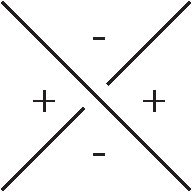
\includegraphics[width=.4\textwidth]{figs/cornerasy.pdf}
  \caption{Quadrants near a crossing in $\pi(L).$}
  \label{fig:quad_sign}
\end{figure}

\subsection{The \Ainf-maps $m_k$}
\label{sect:Ainf_m}
% Now we mey define the \Ainf-maps.

Fix $k$, and let $a, b_1, ...,  \in \Cc$, then denote
\[ \M^a_{b_1...b_k} = \{ u \in W^+(Y,a) \q|  u(x^k_i) = b_i \text{ for } i\ge 1 \}. \]
Then define
\[ m_k(b_1, ..., b_k) := \sum_{a\in\Cc} (\#_2 \M^a_{b_1...b_k}) a, \]
where $\#_2$ denotes the number of elements modulo 2, which is well-defined, by
lemma \pref{prop:W_+_finite}.

\begin{them}[Chekanov 2002, \cite{chekanov02}]
\label{prop:a_inf_rels}
The maps $m_k$ have degree $2-k$ and satisfies the curved $A_\infty$-relations,
ie. $\forall n\ge 0$,
\begin{equation}
\label{eq:a_inf_rel}
\xi_n := 
\sum_{r+s+t = n} m_u(\I^{\otimes r} \otimes m_s \otimes \I^{\otimes t})  = 0,  
\end{equation}
where $u = r+1+t$. Hence, by lemma \pref{prop:W_+_finite}, $(A,m_i)$ defines a
finite curved $A_\infty$-algebra.
\end{them}

\begin{them}[Chekanov 2002, \cite{chekanov02}]
\label{prop:stable_tame_inv}
Let $(A,m)$ and $(A', m')$ be the \Ainf-algebras associated to Legendrian knots $L$ and $L'$. Then if $L$ and $L'$ differ by a Legendrian isotopy, $(A,m)$ and $(A',m')$ have the same sable type.
%are related by a stable tame isomorphism.
\end{them}

The proofs of these theorems are given in chapter \ref{chap:proofs}.


    
    \section{Examples}
    
% https://services.math.duke.edu/~ng/knotgallery.html

We will start by computing the \Ainf algebra associated with the Legendrian
projection of some very simple knots shown in figure \ref{fig:simple_knots}. 

\begin{figure}
\centering
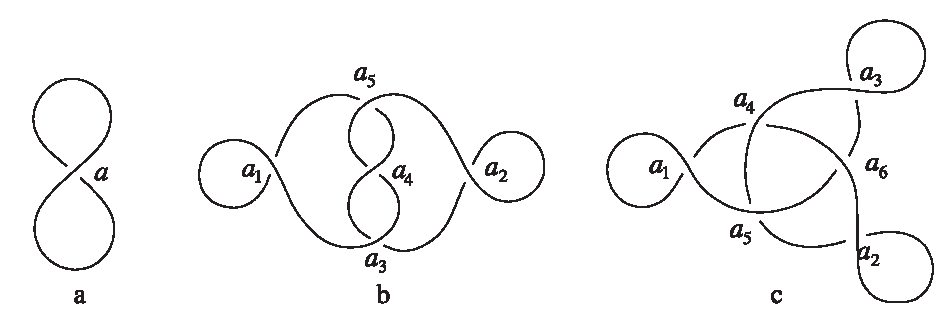
\includegraphics[width=.8\textwidth]{figs/simple_knots.pdf}
\caption{$k$ sided polygon.}
\label{fig:simple_knots}
\end{figure}

\begin{exmp} Let $Y_0$ be the Lagrangian projection of the Legendrian unknot
$L_0$, shown figure (\ref{fig:simple_knots}a). The winding number $\sigma(L_0) =
0$, so the grading takes values in $\Gamma = \Z$. There is only one crossing
$a$, with degree $|a| = 1$. So $A = \Z_2\<{a}$. The set of immersions
$\tilde{W}_k(Y_0)$ is empty for $k > 1$ and $\tilde{W}_k(Y_0) = \{ f_1, f_2 \}$,
where $f_1$ and $f_2$ are the immersions whose image are the two bounded
components of $\R^2 \setminus Y_a$. Considering the sign of the quadrants of the
crossing, we observe that both $f_1$ and $f_2$ are admissible. Hence $m_k = 0$
for all $k>0$ and $m_0(1) = \#_2\{f_1,f_2\} a = 0$.
\end{exmp}

\begin{exmp}
Consider $Y_r$ given by figure (\ref{fig:simple_knots}b), the Lagrangian
projection of the Legendrian Right-handed trefoil knot $L_r$. The winding number
$r=0$ again, so $\Gamma = \Z$. There is $5$ crossings, $A = \<{b_1, b_2, b_3,
a_1, a_2}$, and the grading is given by
\[ |a_i| = 1, \quad |b_i| = 0. \]
There is two admissible immersions with one vertex, there is also four with two
vertices and two with four (see figure \ref{fig:simple_knots}b). So $m$ is given
by

\begin{align*}
m_0(1) = m_1(b_1) = m_1(b_3) &= a_1 + a_2 \\
m_3(b_1,b_2,b_3) &= a_1 \\
m_3(b_3,b_2,b_1) &= a_2.
\end{align*}
And all other terms are zero.

\end{exmp}


We will also have a look at two other slightly more complicated knots, shown in
figure \ref{fig:chek_elias_knots}. Later we will see that with the invariant
induced by the associated \Ainf algebra one are able to distinguish this two
knots, even though both knots has the same classical invariants.

\begin{figure}
\centering
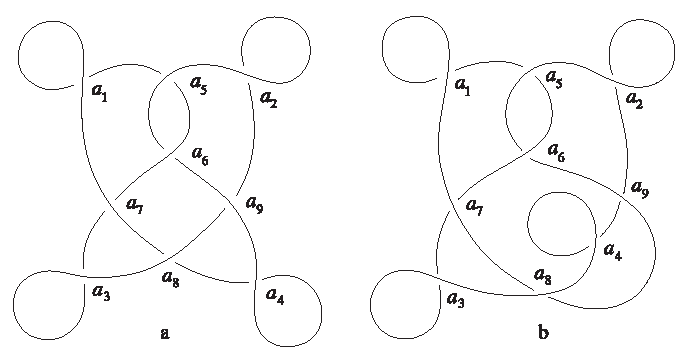
\includegraphics[width=.8\textwidth]{figs/chek_elias_knots.pdf}
\caption{$k$ sided polygon.}
\label{fig:chek_elias_knots}
\end{figure}

\begin{exmp}
Let $Y_a$ and $Y_b$ be given by figure (\ref{fig:chek_elias_knots}). 
For both of the knots the winding number $r=0$ and there is $9$ crossings,
enumerated as shown in the figure. Let's first consider diagram (a), the grading
is given by
\[ |a_i| = 1, \quad |a_5| = 2, \quad |a_6| = -2 \q\tand |a_j| = 0, \]
where $i = 1,...,4$ and $j = 7,...,9$. The \Ainf maps $m_i$ is given by

\begin{align*}
m_0(1) &= a_1 + a_2 + a_3 + a_4, \\
m_3(a_7,a_6,a_5) = m_1(a_7) &= a_1, \\
m_3(a_5,a_6,a_9) = m_1(a_2) &= a_2, \\
m_2(a_8,a_7) &= a_3, \\
m_2(a_9,a_8) &= a_4.
\end{align*}
And all other terms are zero. Now les's consider the second diagram. The grading
is given by
\[ |b_i| = 1 \q\tand |b_j| = 0, \]
where $i = 1,...,4$ and $j = 5,...,9$. The \Ainf maps are given by

\begin{align*}
m_0(1) &= b_1 + b_2 + b_3 + b_4, \\
m_3(b_7,b_6,b_5) = m_1(b_7) &= b_1, \\
m_3(b_9,b_8,b_5) = m_1(b_5) &= b_1, \\
m_3(b_5,b_6,b_9) = m_1(b_9) &= b_2, \\
m_2(b_8,b_7) &= b_3, \\
m_2(b_9,b_8) &= b_4.
\end{align*}
And all other terms are zero. So clearly this are different \Ainf algebras, but
that is not in itself a sufficent argument for to say that they are different
knots.

\end{exmp}

    
    %%%%%%%%%%%%%%%%%%%%%%%%%%%%%%
    \chapter{The Chekanov invariant}

    \section{Maurer-Cartan elements and the Chekanov-Poincar\'{e} polynomials}
    
% \subsection{The Chekanov-Poincar\'{e} polynomials}

Consider a finite \Ainf-algebra $(A,m)$ over $\Z_2$. If $A$ in uncurved, recall that we may define the cohomology 
\[ H^*(A, m_1) = \frac{\ker m_1}{\im m_1}, \] 
a $\Gamma$ graded $k$-vector space. 

\begin{defn}
If $A$ is uncurved and finite-dimensional then so is the cohomology, so we may define the \wddef{Poincar\'{e} Polynomial}
\[ P_A(\lambda) := \sum_{i \in \Gamma} \dim\qty( H^i(A,m_1) )\cdot \lambda^i. \]
\end{defn}

This is clearly a invariant of the cohomology of uncurved \Ainf algebras. However
is is not clear how this is useful as an invariant of Legendrian knots, as the
associated \Ainf algebra in general is curved.



% \subsection{Maurer-Cartan element}

\begin{defn}
Let $a \in A$, then, for $n \in \N$, define 
$ m^c: TA \to A, $by 
\begin{equation}
\label{eq:def_id_of_mc}
m^c_n(a_1,...,a_n) := \sum_{i_0,...,i_n}
m_u\big(\underbrace{c,...,c}_{i_0},a_1,\underbrace{c,...,c}_{i_1},a_2,c,...,c,a_n,\underbrace{c,...,c}_{i_n}\big), 
\end{equation}
where the sum runs over all combinations of $i_0,...,i_n \ge 0$.
\end{defn}

Note that, since $A$ is finite, the sum is well-defined.
Also note that from here on, we will write $c...$, to mean a sequence of $c$'s. If we write $c,...,c$, the dots might also contain more then
just $c$'s.

\begin{lemma}
\label{prop:Ac_is_ainf}
If $|c| = 1$, then $A^c := (A, m^c)$ defines a new finite curved \Ainf-algebra
\end{lemma}

\begin{proof}
First we need $|c| = 1$, in order for the maps to have the correct degree. With
$|c|=1$ this works out, since the degree increases by 1 for each occurrence of $c$
and decreases by 1 for each extra entry in $m_u$.  
It is immediately clear from the definition that it is finite, so it suffuses to
check that the \Ainf-relations hold.

\begin{align*}
&\sum_{r,s,t} m^c_u (a_1,...,a_r, m^c_s(a_{r+1},...,a_{r+s}), a_{r+s+1},...,a_{n}) \\
&= \sum_{r,s,t} \sum_{i_0,...,i_s} m^c_u (a_1,...,a_r, 
m_{u'}(\underbrace{c...}_{i_{0}},a_{r+1},c,...,c,a_{r+s},\underbrace{c...}_{i_{s}})
a_{r+s+1},...,a_{n})\\
&= \sum_{r,s,t} \sum_{i_0,...,i_s} \sum_{j_0,...,j_{u}} m_{u''} (\underbrace{c...}_{i_0},a_1,c,...c,a_r,\underbrace{c...}_{j_r}, \\
& \qquad\qquad 
m_{u'}(\underbrace{c...}_{i_0},a_{r+1},c,...,c,a_{r+s},\underbrace{c...}_{i_{r+s}}),
\underbrace{c,...}_{j_{r+1}},a_{r+s+1},c,...,c,a_{n},\underbrace{c...}_{j_u}) \\
% &= \sum_{N\ge n} \sum_{r,s,t} \sum_{i_*,j_*} \qty\{\text{same as in the previous line} \}
\end{align*}
In the first line we expand the inner $m^c$ according to
(\ref{eq:def_id_of_mc}), and in the second line we expand the outer $m^c$. The
indices $r,s,t$ are as in the \Ainf-relations (\ref{eq:Ainf_rels}) and the
indices $i_0,...,i_s$ and $j_0,...,j_u$ are as in (\ref{eq:def_id_of_mc}).
Finally $u=r+t+1$, $u' = s + \sum i_k$ and $u'' = r+t+\sum j_k$. (Note that, for
now on, this indices will be assumed without stated explicitly. ) 

Considering the sums in the last line, we can sort them according to the total
number of $c$'s (ie. $N = \sum_k i_k + \sum_k j_k)$. 
\[ \sum_{r,s,t} \sum_{i_0,...,i_s} \sum_{j_0,...,j_{u}} \{ ... \}
= \sum_{N \ge 0} \sum_{r,s,t} \sum_{i'_0,...,i'_s} \sum_{j'_0,...,j'_u} \{
... \}. \]
Then for each $N$ the inner sum is the left hand side of the $N$'th \Ainf-relation in $m$ applied to $\xi_N \in A^{\otimes N}$, the sum of all ways of putting $N$ $c$'s between the $a$'s. ie.
\[  \xi_N = \sum_{k_0,...,k_n} (\underbrace{c...}_{k_0}, a_1, c,...,c, a_n,
\underbrace{c...}_{k_n}),
\qquad k_0+...+k_n = N. \] 
Since the $m$ satisfy the \Ainf-relation, we are done.
\end{proof}

\begin{defn}
An element $c \in A$ is called a \wddef{Maurer-Cartan element} (MC element) if $|c| = 1$ and 
\[ \sum_{n \ge 0} m_n(c...) = 0. \]
\end{defn}

\begin{lemma}
$(A,m^c)$ is uncurved if and only if $c$ is a MC element.
\end{lemma}

\begin{proof}
By definition,
\[ m_0^c = \sum_{n \ge 0} m_n(c...) = 0 \]
\end{proof}

\begin{defn}
If $A$ is a finite-dimensional finite curved \Ainf-algebra, define 
\[ I(A) := \{ P_{A^c} \q: c \in A \text{ is a MC element} \}. \]
\end{defn}

We later will see that this set of Poincar\'{e} polynomials is invariant under
stable tame isomorphism and thus Legendrian isotopy. Not that the isomorphism
need not actually be tame, for this to be true. 

\begin{defn}
\label{def:hom_c}
Let $c \in A$ and $f: A \ato B$, then like in (\ref{eq:def_id_of_mc}), define
$f_n : A^{\otimes n} \to B$ by
\begin{equation}
\label{eq:hom_c}
f^c_n(a_1,...,a_n) := \sum_{i_0,...,i_n}
f_u(\underbrace{c...}_{i_0},a_1,c,...,c,a_n,\underbrace{c...}_{i_n}).
\end{equation}
Also, we write $f_*(c) := f_0^c = \sum_{n\ge 0} f_n(c...)$.
\end{defn}

\begin{lemma}
If $f: A \ato B$ and $c\in A$ is a MC element, then so is $f_*(c) \in B$.
\end{lemma}
\begin{proof}
By the defining relation of $f$ (\ref{eq:ainf_morph_rel}) and linearity we
have.
\begin{align*}
m^B_n(f_*(c), ..., f_*(c)) 
&= \sum_{i_1,...,i_n} m^B_n(f_{i_1}(c...), ..., f_{i_n}(c...)) 
= \sum_{r,s,t} f_u(c..., m_s(c...), c...)  \\
&= \sum_{r,t} f_u(c..., \sum_s m_s(c...), c...)  = 0
\end{align*}
\end{proof}

\begin{lemma}
$\{ f^c_n \}_{n \ge 1}$ defines a finite uncurved \Ainf-homomorphism 
\[ f: A^c \to B^{f_*(c)}. \]
\end{lemma} 

\begin{proof}
We need to check that $f$, satisfy equation (\ref{eq:ainf_morph_rel}). 
We have
\begin{align*}
& \text{LHS} (a_1,...,a_n) \\
&= \sum_{r,s,t} f^c_u (a_1, ..., a_r, m^{A,c}_s(a_{r+1}, ..., a_{r+s}),
a_{r+s+1}, ..., a_{n}) \\
%
% &= \sum_{r,s,t} \sum_{i_1,...,i_s} f^c_u (a_1, ..., a_r, m_s(c...,a_{r+1}, c,
% ...,c, a_{r+s},c...),
% a_{r+s+1}, ..., a_{n}) \\
%
&= \sum_{r,s,t} \sum_{i_0,...,i_s}\sum_{j_0,...,j_u} 
f_u \big(\underbrace{c...}_{j_0},a_1,c,...,c, a_r,\underbrace{c...}_{j_r}, \\
& \qquad\qquad\qquad\qquad\qquad 
m^A_s(\underbrace{c...}_{i_0}, a_{r+1}, c,...,c, a_{r+s},\underbrace{c...}_{i_s}),
c..., a_{r+s+1},c..., a_{n} \big) 
\end{align*}
The first line is precisely what appear in the equation. In the following line
we expand $m^c$ and $f^c$. Like in the proof of lemma (\ref{prop:Ac_is_ainf}),
we sort the terms according the total number of $c$'s. We get the left hand
side of the $N$th \Ainf-homomorphism relation in $f$ and $m$, applied to $\xi_N \in
A^{\otimes N}$ (where $\xi$ is as in lemma (\ref{prop:Ac_is_ainf})). Applying
the relation we have
\begin{align*}
& \text{LHS} (a_1,...,a_n) 
= \sum_N \sum_{i_1,...,i_r} m^A_r (f_{i_1} \otimes ... \otimes f_{n}) (\xi) \\
&= \sum_N \sum_{i_1,...,i_r} \sum_{k_0,...,k_n} m^A_r (f_{i_1} \otimes ... \otimes
f_{i_r}) (\underbrace{c...}_{k_0}, a_1, c,...,c, a_n,
\underbrace{c...}_{k_n})
\end{align*}
Now, let's also study the right hand side.
\begin{align*}
&\text{RHS} (a_1,...,a_n) \\
&= \sum_{i_1,...,i_r} m^{B,f_*(c)}_r (f^c_{i_1}(a_1,...,a_{i_1}), ...,
f^c_{i_r}(a_{n-i_r},...,a_n)) \\ 
&= \sum_{i_1,...,i_r}\sum_{k_0,...,k_s} m^B_r
(f_{i_1}(\underbrace{c...}_{k_0},a_1,c,...,c,a_{i_1},\underbrace{c...}_{k_{i_1}}), ...,
f_{i_r}(\underbrace{c...}_{k_{s-i_r}},a_{n-i_r},c...,a_n,\underbrace{c...}_{k_s})) 
\end{align*}
where $s = r + \sum i_*$. It is quite clear that these sums agree and thus we
are done.  
\end{proof}


% \begin{lemma}
% $c \in A$ is a MC element if an only if the map $\epsilon: T(A^*) \to k$, given by $\epsiolon(\alpha_1\otimes ... \otimes \alpha_n) = \alpha_1(c)\cdot ... \cdot \alpha_n(c)$, is an augmentation.
% \end{lemma}

\begin{lemma}
Let $f: B \ato C$ and $g: A \to B$, then for any MC element $c \in A$, 
$(f\circ g)^c = f^{g_*(c)} \circ g^c$ and in particular 
$(f \circ g)_* (c) = f_*(g_*(c))$.
\end{lemma}

\begin{proof}
\begin{align*}
&(f_{g_*(c)} \circ g_c)_n (a_1, ..., a_n) \\
&= \sum_{i_1,...,i_r} f^{g_*(c)} ((g_c)_{i_1}(a_1,...,a_{i_1}), ...,
(g_c)_{i_r}(a_{n-i_r},...,a_n)) \\
&= \sum_{i_1,...,i_r}\sum_{j_0,...,j_s} 
f (\underbrace{g_*(c)...}_{j_0 \text{ times}},(g_c)_{i_1}(a_1,...,a_{i_1}), 
g_*(c),...,g_*(c), (g_c)_{i_r}(a_{n-i_r},...,a_n), 
\underbrace{g_*(c)...}_{j_s}) 
\end{align*}
Here the first equality follows from expanding the definition of the
composition. So the sum in $i$ runs over all $i$'s such that $i_1+...+i_r = n$.
The second equality, follows from the expanding of the definition of $f^c$.
Note the notation $\alpha...$, means $\alpha$ is repeated some number of times.

\begin{align*}
&(f \circ g)^c_n (a_1, ..., a_n) \\
&= \sum_{i_1,...,i_n} (f \circ g)_n (\underbrace{c...}_{i_0},a_1,c,...,c,a_n,
\underbrace{c...}_{i_n}) \\
&= \sum_{i_1,...,i_n}\sum_{j_1,...,j_s} 
f_s(
\lefteqn{\underbrace{\phantom{\overbrace{c,...,c}^{\text{apply }g_{j_0}},c...,
c...}}_{i_0}} 
\overbrace{c,...,c}^{\text{apply }g_{j_0}},c..., 
\overbrace{c...,a_1,c,...,c,a_*,c...}^{g_{j_*}}, 
\overbrace{c,...,c}^{g_{j_{*}}}, ... , 
\overbrace{c...,a_n,c...}^{g_{j_*}},..., 
\overbrace{c,...,c}^{g_{j_s}} ) \\
%%
&= \sum_{k_1,...,k_r}\sum_{l_0,...,l_s} 
f (\underbrace{g_*(c)...}_{j_0},(g_c)_{i_1}(a_1,...,a_{i_1}), 
g_*(c),...,g_*(c), (g_c)_{i_r}(a_{n-i_r},...,a_n), 
\underbrace{g_*(c)...}_{j_s}) 
\end{align*}
In the first line we expand $(f\circ g)^c$ according to def. (\ref{def:hom_c}).
And in the second line we expand the composition, where the underbraces indicate
applying $g$ to the indicated elements. On the last line we recognise the
definition of $g_c$ and $g_*$ in the previous line and re-index accordingly.
\end{proof}

\begin{corol}
If $f: A \ato B$ is a finite uncurved \Ainf-isomorphism, 
then for any MC element $c \in A$, 
%
\[ (f^c)^*: H^*(A, m_1^{A,c}) \to H^*(B, m_1^{B,f_*(c)}) \]
is an isomorphism.
\end{corol}

\begin{proof}
We have
\[ A^c \xrightarrow{f^c} B^{f_*(c)} \xrightarrow{g^{f_*(c)}}
A^{g_*(f_*(c))} = A^c,  \]
where the equality follows from the lemma above. Also, by the lemma above 
\[ g^{f_*(c)} \circ f^c = (g \circ f)^c = \id_A^c = \id. \]
Similarly $f^c \circ g^{f_*(c)} = \id_B$. So by lemma
(\ref{prop:Ainf_iso_induced}), the result follows.
\end{proof}

\begin{lemma}
If $f: A \ato B$ is an \Ainf-isomorphism, then $I(A) = I(B)$.
\end{lemma}

\begin{proof}
If $c \in A$ is a MC element, $f_*(c) \in B$ is an MC element and 
\[ (f^c)^* : H^*(A, m_1^{A,c}) \to H^*(B, m_1^{B,f_*(c)}) \]
is an isomorphism, and thus 
\[ P_{A^c} = P_{B^{f_*(c)}}. \]
Therefore $I(B) \subseteq I(A)$. By applying the same argument with
$g^{(f_*(c))}$, \\ $I(A) \subseteq I(B)$ and the result follows. 
\end{proof}

Now, the only thing we have left in order to show that $I(A)$ is a Legendrian
knot invariant. That is % invariance under stabilication.

\begin{lemma}
$I(A) = I(S_i(A)).$
\end{lemma}

\begin{proof}
Let $c \in A$ be a MC element. 
Then $c \oplus 0 \in A \oplus k\<{e_1,e_2}$ is a MC element in $S_i(A)$.
Since clearly $|c\oplus 0| = |c|= 1$ and 
\[\sum_{n\ge 0} m^{S_i(A)}_n((c\oplus 0)...) = \sum_{n\ge 0} m^A_n(c...) = 0.\]

Also, it follows easily from the definition of the stabilization that
$m^{S_i(A), c}_1 (a) = m^{A,c}_n (a)$ for all $a \in A$ and $m^{S_i(A),
c}_1(e_j) = m^{S_i(A)}_1(e_j)$. So, since $m^{S_i(A)}_1(e_1) = e_2$ and
$m^{S_i(A)}_1(e_2) = 0$, 
\[ \im m^{S_i(A), c}_1 = \im m^{A,c}_1 \oplus \im e_2 
\qq{\text{and}} [e_1] = [0] \in H^*(S_i(A), m^{S_i(A),c}_1). \].
So 
\[ H^*\qty(S_i(A), m^{S_i(A),c}_1) = H^*(A, m^{A,c}_1) \]
Thus $I(A) \subseteq I(S_I(A))$. 

Now for the reverse inclusion, suppose $c \oplus (\alpha e_1 + \beta e_2) \in S_i(A)$ is a
MC element for some $c\in A$, $\alpha, \beta \in k$. Then 
\[ 0 = \sum_{n \ge 0} m^{S_i(A)}_n \qty(c \oplus (\alpha e_1 + \beta e_2)...) =
\qty( \sum_{n \ge 0} m^A_n(c...) ) \oplus \alpha e_2. \]
So $\alpha = 0$ and $c \in A$ is a MC element. 

As above it is easy to check that 
\[ H^*\qty(S_i(A), m^{S_i(A),c\oplus \beta e_2}_1) = H^*(A, m^{A,c}_1). \]
Hence $I(A) \supseteq I(S_I(A))$.
\end{proof}

It then follows directly from two lemmas above that.
\begin{them}
$I(A)$ an invariant of stable type and thus, by theorem
(\ref{prop:stable_tame_inv}), a Legendrian knot invariant.
\end{them}

Note that the tame \Ainf-isomorphism condition, in the definition of the stable type,
is not necessary for this theorem to hold. Instead an finite \Ainf-isomorphism
would suffice.

% \subsection{Examples}

% With wich we can conclude that there exist non-isotopic legendrian knots with the same clasical invariances.




    \section{Examples} %%% TODO
    \todo{Calculate $I(A)$ for the check-elias-knots.}
 
    %%%%%%%%%%%%%%%%%%%%%%%%%%%%%%
    \chapter{The Proofs}
    \label{chap:proofs}

    In this chapter we will takel the proof of the two most centereal theorems in
this paper. Theorem \pref{prop:a_inf_rels} and \pref{prop:stable_tame_inv}. 
Since we are spesificly working with the standard contactstructure on $\R^3$ and
more spesificly the lagrandian projection, the proofs will nauturaly reduce to a
combinatorial agrument.

Throught this chapter we will consider a fixed but arbitrary Legendrian knot
$L$ and it's Lagrangian projection $Y = \pi(L)$.

Both of the proofs, including the lemmas presente in the first section is an
adoptation of the the proofs given in \cite{chekanov02}. (Addapted to the
language of \Ainf-algebras.)

 
    \section{Preliminary Lemmas}
    
% Consider a crossing $c \in \Cc(Y)$, then like when we defined the grading observe that there exists unique $c_+, c_- \in L$, such
% that $\pi(c_+) = \pi(c_-) = c$ and $z(c_+) > z(c_-)$. 

Consider a crossing $c \in \Cc(Y)$, then like when we defined the grading,
let $c_+, c_- \in L$, such $\pi(c_+) = \pi(c_-) = c$ and $z(c_+) > z(c_-)$.

\begin{defn}
Definie the the height map 
\[ H : \Cc(Y) \to  \R^+, \]
by 
$ H(c) = z(c_+) - z(c_-)$, for all $c \in \Cc$.
\end{defn}

% This lemma is needed for the proof of d^2 = 0.

\begin{lemma}
\label{prop:l_6.1}
Let $u \in W_k(Y)$. Then 
\[ \sum_{x \in Q_+} H(u(x)) - \sum_{x\in Q_-} H(u(x)) = \int_{\Pi_k} u^*(\d y \wedge \d x) > 0, \]
where $Q_+$ (resp. $Q_-$) is the set of positive (resp. negative) vertices for $u$. In particular, at least one of the vertices of $\Pi_k$ is positive.
\end{lemma}

\begin{proof}
Consider the integral $I = \int_{u(\partial \pi_k)} y \d x$. Then, by Stoke's theorem, we have
\[ I = \int_{\Pi_k} u^*(\d y \wedge \d x) > 0, \]
where the inequality is due to $u$ beeing orientation preserving.

Let $X_i \subset \partial \Pi_i$ denote the edge connection $x^k_i$ and $x^k_{i+1}$,
where $0\le i\le k-1$. Let $\gamma_i : X_i \to L$, such that 
\[ \pi \circ \gamma_i = u|_{X_i}. \] 
Since $\partial \Pi_k = \bigsqcup_i X_i$, we have 
\[ I = \sum_i \int_{\gamma_i(X_i)} y \d x. \]
Also for all $i$, $\gamma_i$ is a legendrian curve, ie. 
$\gamma_i'(d) \in \ker ( \d z - y \d x )$. So
\[ I = \sum_i \int_{\gamma_i(X_i)} \d z. \]

For each $i$, let $\sigma: [0,1] \to \R^3$ be a
parameterisation of the vertical line
segment connecting $z_+(u(x^k_i))$ with $z_-(u(^k_i))$ (ie. $\pi \circ
\sigma_i$ is constent at $u(x^k_i)$,) oriented from $z_-$ to $z_+$ if $x^k_i$ if positive for $u$ and from $z_+$ to $z_-$ if $x^k_i$ is negative for $u$. 

By assosiating $X_i$ with the unit interval, oriented from $x^k_i$ to
$x^k_{i_+1}$ we concatenate the curves into one closed curve, 
$\Gamma = \gamma_0 \star \sigma_0 \star ... \star \gamma_{k-1} \star
\sigma_{k-1}$. 
Since $\Gamma$ is closed, $\int_\Gamma \d z = 0$. Hence 
%
\[ I = \sum_i \int_{\gamma_i(X_i)} \d z - \int_\Gamma \d z = -\sum_i
\int_{\sigma{[0,1]}} \d z \quad = LHS.  \]
\end{proof}
%
The following corolary follows immideatly.
\begin{corol}
\label{prop:height_sum}
If $u \in W^+(Y)$ then $H(u(x^k_0)) \ge \sum_{i=1}^{k-1} H(u(x^k_i))$.
\end{corol}

% \begin{proof}[proof of lemma \pref{prop:W_+_finite}]
\subsubsection{proof of lemma \pref{prop:W_+_finite}}
Consider the complement of $L$ in $\R^2$. Then for some indexing set $I$, let
$\{U_i\}_{i\in I}$ denote the set of connected components, ie. $U_i$ is
connected for each $i\in I$ and 
\[ \bigcup_{i \in I} U_i = \R^2 \setminus L. \]
Since $L$ is compact, clearly $I$ is finite. Let $I = \{0,1,...,m\}$ and suppose
$U_0$ is the unbounded component.  

Let $S_i$ be the area of $U_i$, then 
\[ \int_{\Pi_k} f^*(\d y \wedge \d x) = \sum_{i=1}^n n_i(f) S_i, \] 
where the integer $n_i(f) \ge 0$ equal to the cardinality of
$f^{-1}(z)$, for $z \in U_i$.

It follows from from the corollary above that $\sum_{i=1}^m n_i(f) S_i$ is
bounded above by $\max_{c\in \Cc} H(c)$. Since $S_i > 0$, there are only finitely many
ways of choosing the coefficients $n_i$. Also, for a fixed sequence $n_1, ...,
n_m$, there are clearly only finitely many admissible immersions $f$, such that
$n_i(f) = n_i$. Hence, the total number of admissible immersions is finite.
\qed %\end{proof}

% This lemma is needed for the proof of the invariance under the Reidemeister moves
\begin{lemma}
\label{prop:deg_sum}
Let $u \in \tilde{W}_k (Y)$. Then 
\[ \sum_{x \in Q_+} \deg(u(x)) - \sum_{x \in Q_-} \deg(u(x)) = 2 - |Q_-|, \]
where $Q_+$ (resp. $Q_-$) is the set of positive (resp. negative) vertices with respect to $f$.
\end{lemma}

Note that it follows from the particular case of $|Q_+| = 1$, that the
\Ainf-maps $m_k$ has degree $2 - k$. 

\begin{proof}
Like in the proof of \pref{prop:l_6.1}, let $X_i \subset \partial \Pi_k$ be the
edge connecting $x^k_i$ and $x^k_{i+1}$. 
Consider the smooth immersions $\rho_i : X_i \to L$, such that $f|_{X_i} = \pi
\circ \rho_i$. Let $y_i = \rho_i(x^k_i)$, $y'_{i+1} = \rho_i(x^k_{i+1})$ and
$y'_0 = y'_k$, for $0 \le i \le k-1$. Then let
\[ C_1 = \sum_{i=0}^{k-1} \theta(y_i, y'_{i+1}) \qq{\text{and}}
   C_2 = \sum_{i=0}^{k-1} \theta(y'_i, y_i),  \]
where $\theta : L \times L \to \Gamma$ is the map from definition
\pref{def:theta_map}.

Then, by the additivity of $\theta$, $C_1 + C_2 = 0$ mod $m(L)$. Also $C_1 = 2 r(K)$, where $r(K)$ is the rotation
number of the closed curve $K = u(\partial \Pi_k)$ (defined as the sum of
the rotation numbers of its smooth pieces). Let $\phi_i$ denote the exterior
angle of the crossing at $u(x^k_i)$, where exterior refers to the
angle of a quadrant adjacent to the one covered by $u$, see figure
\pref{fig:outer_angle}.

\begin{figure}
\centering
% \definecolor{qqwuqq}{rgb}{.2,.2,.2}
% \definecolor{zzttqq}{rgb}{.3,.3,.3}
% \begin{tikzpicture}[line cap=round,line join=round,>=triangle 45,x=5cm,y=5cm]
% \clip(-.1,-.1) rectangle (2,2);
% \fill[line width=2pt,color=zzttqq,fill=zzttqq,fill opacity=0.1] (0,0.07) -- (0.43,0.5) -- (0,0.93) -- cycle;
% \draw [shift={(0.5,0.5)},line width=2pt,color=qqwuqq,fill=qqwuqq,fill
% opacity=0.1] (0,0) -- (45:0.427) arc (45:135:0.427) -- cycle;
% \draw [line width=2pt] (0,0)-- (1,1);
% \draw [line width=2pt] (0,1)-- (0.45,0.55);
% \draw [line width=2pt] (0.55,0.45)-- (1,0);
% \draw [line width=2pt,color=zzttqq] (0,0.07)-- (0.43,0.5);
% \draw [line width=2pt,color=zzttqq] (0.43,0.5)-- (0,0.93);
% \draw (0.014,0.6) node[anchor=north west] {$u(\Pi_k)$};
% \draw (0.449,0.856) node[anchor=north west] {$\phi_i$};
% \end{tikzpicture}
% 
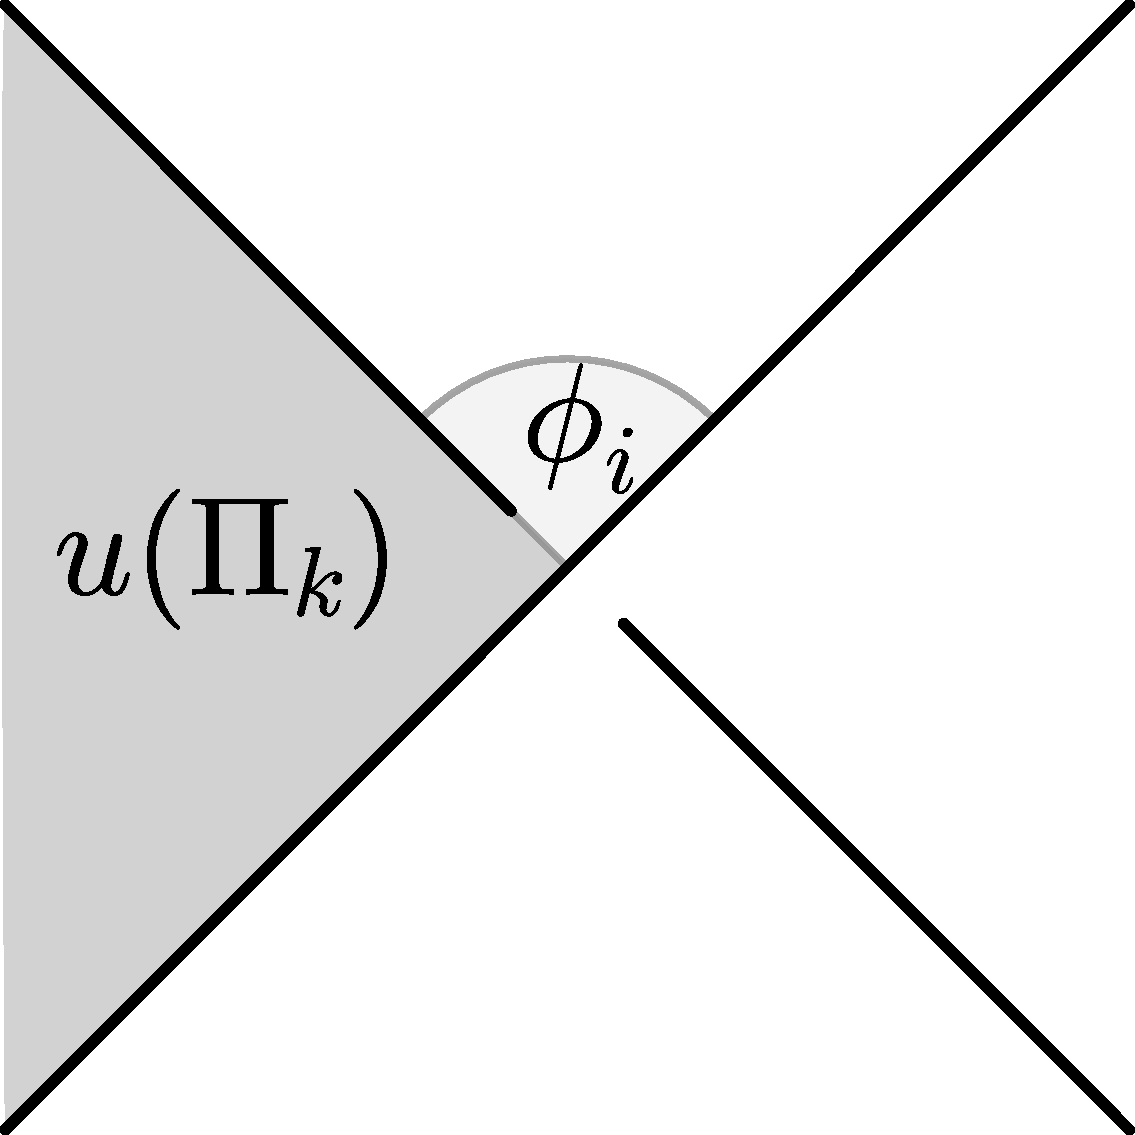
\includegraphics[width=.25\textwidth]{figs/outer_angle.pdf}
\caption{The exterior angle $\phi_i$.}
\label{fig:outer_angle}
\end{figure}

Then $r(K) = 2 - \sum \phi_i$ and thus $C_2 = -C_1 = 2\sum \phi$. Also,
\[ |u(x^k_i)| = \lceil \theta\qty(z^+_i, z^-_i) \rceil = \pwf{ - \theta_i + \phi_i  &\tif x_i  \in Q_+ \\
Q_i + (1 - \phi_) &\tif x_i \in Q_-.}  \]
By defining the sign $\mu_i$, given by $\mu_i = \mp1$ if $x_i \in Q_\pm$, we can
write 
\[ |u(x^k_i)| = \mu \theta_i - \mu_i + \frac{1+\mu_i}{2}. \]
Then, using $\mu_i^2 = 1$,
\[ LHS = - \sum \mu_i |f(x_i)| = \sum (\theta_i - \phi_i +
\frac{1+\mu_i}{2}) = -(-2 + |Q_-|).   \]

\end{proof}



    
    \section{Proof of theorem (\ref{prop:a_inf_rels})}
    % Proof of A_inf relations

The proof here is essentially the same as that of Theorem 3.3 in chapter 7
[\cite{chekanov02}]. The magare differece is found in the fist subsection, in
which we reduce the algebraic problem to a combinatoiral one.

\subsection{Plan of the proof}

By the linearity of (\ref{eq:a_inf_rel}), it suffuses to show that it is
satisfied when applied on the generators. That is 
\[
\xi_n(a_1,...,a_n) = \sum_{r+s+t = n} m_u(a_1,...,a_r, m_s(a_{r+1, ..., r+s}), a_{r+s+1}, ..., a_n)  = 0,  
\]
for all $a_1, ..., a_n \in \Cc$ (and $u = r+1+t$, like before.)

To show that relation hold, we will show every term in $\xi_n$ occur an even
number of times and thus cancel out, since we are working over $\Z/2\Z$. 

First consider one term in the sum, ie. for a fixed $r,s,t$, such that
$r+s+t=n$. 
Then

\begin{align*}
m_u(a_1,..., a_r, &m_s( a_{r+1}, ..., a_{r+s} ), a_{r+s+1}, ..., a_n) \\
% &= m_u(a_1,...,a_r, \sum_{a\in\Cc} (\#_2 \M^a_{a_{r+1}...a_{r+s}}) a, a_{r+s+1}, ..., a_n )
&= \sum_{a\in\Cc} (\#_2 \M^a_{a_{r+1}...a_{r+s}}) m_u(a_1,...,a_r, a, a_{r+s+1}, ..., a_n ) \\
&= \sum_{a\in\Cc}\sum_{b\in\Cc} (\#_2 \M^a_{a_{r+1}...a_{r+s}}) (\#_2 \M^b_{a_1,...,a_r, a, a_{r+s+1}, ..., a_n}) b \\
&= \sum_{b\in\Cc} Z_{r,s,t}(b,a_1, ..., a_n) b,
\end{align*}
%
where $Z_{r,s,t}(b,a_1,...,a_n)$ is the number of triplets $(u',a,u'')$, such that 
%
\newcommand{\kp}{{k'}}
\newcommand{\kpp}{{k''}}

\begin{itemize}
\item 
$u' \in W^+_\kp(Y,b), \quad a\in \Cc, \quad u'' \in W^+_\kpp(Y,a) $;
\item
$\left( u'(x^\kp_1), ..., u'(x^\kp_{u-1}) \right) = \left(a_1,...,a_r, a, a_{r+s+1}, ..., a_n\right)$
\item
$\left(u''(x^\kpp_1), ..., u''(x^\kpp_s) \right) = \left(a_{r+1},...,a_{r+s}\right)$.
% \item 
% $(a_1,...,a_n) = ( u'(x^\kp_1), ..., u'(x^\kp_r), u''() ) $
\end{itemize}
\figpdf{.4}{splitting}
{An example of a triplet $(u',a,u'') \in U_{1,4,1}(b,a_1,...,a_6)$.}

Here $\kp = u+1$ and $\kpp = s+1$. For an example see figure \pref{fig:splitting}. Let $U_{r,s,t}(b,a_1,...,a_n)$ denote the set of such triplets. Note that for $(r',s',t') \ne (r,s,t)$, 
\[ U_{r,s,t}(b,a_1,...,a_n) \cap U_{r',s',t'}(b,a_1,...,a_n) = \emptyset, \]
so we can conclude that 
\[ \xi_n(a_1,...,a_n) = \sum_{b\in\Cc} Z(b,a_1,...,a_n) b, \] 
where $Z(b,a_1,...,a_n)$ is the cardinality of
\[ U(b,a_1,...,a_n) = \bigsqcup_{r+s+t=n} U_{r,s,t}(b,a_1,...,a_n). \] 
(Note that $r,s,t$ is not in general determined by $(u',a,u'')$, ie. there
might be $(u',a,u'')$ might be in multiple $U_{r,s,t}$. So, by the
\textbf{discrete} sum, we meed that the elements in $U(b,a_1,...,a_n)$ are
indexed by $r,s,t$.)
%
Now in order to prove that $\xi_n$ vanish, we will need to show that
$Z(b,a_1,...,a_n)$ is even. To prove this we will introduce a new space 
$V^+(b,a_1,..., a_n)$ and construct maps 
\begin{align*}
\vphi: U(b, a_1, ..., a_n) \to V^+(b, a_1, ..., a_n), \qquad
\psi_1, \psi_2: V^+(b, a_1, ..., a_n) \to U(b, a_1, ..., a_n),
\end{align*}
such that for all $u \in V^+(b, a_1, ..., a_n)$ and $g \in U(b, a_1, ..., a_n)$;
\[     \phi(\psi_1) = \phi(\psi_2) = u,
\quad  \psi_1(g) \ne \psi_2(g),\text{ and} 
\quad  \psi_1(\phi(g) = g\text{ or }\psi_2(\phi(g) = g. \]
Then clearly $|U(b,a_1,...,a_2)| = 2|V^+(b,a_1,...,a_n)|$ and the result follows.
\footnote{Here $|V|$, means the cardinality of a set $V$}

\subsection{Auxiliary definitions}
\newcommand{\hu}{\hat{u}}
The maps above indicates that $U$ splits into two pars of equal size. So let
\[  U(b,a_1,...,a_n) = U^l(b,a_1,...,a_n) \sqcup U^r(b,a_1,...,a_n). \] 
%where a way of $U^l$, is the set of 
Given a triplet $(u',a,u'') \in U(b,a_1,...,a_n)$, let $S'\subset \Pi_\kp$ be a
neighbourhood of $x^\kp_{r+1}$ and $S'' \subset \Pi_\kpp$ a neighbourhood of
$x^\kpp_0$. Then there are two possibly relative positions of $S_1 = u'(S')$ and
$S_2 = u''(S'')$ near the crossing $u'(x^\kp_{r+1}) = u''(x^\kpp_0) = a$, see figure
\pref{fig:S_rel_pos}
\figpdf{.4}{S_rel_pos}{Relative position of $S_1$ and $S_2$.}

\begin{defn}
We'll define the subsets $U^l(b,a_1,...,a_n)$ and $U^r(b,a_1,...,a_n)$ to be the
sets consisting of triplets $(u',a,u'')$, for which $S_1$ and $S_2$ have the
relative position represented on the left and right side of figure
\ref{fig:S_rel_pos} respectively. 
\end{defn}

We will now define $V^+(b,a_1,...,a_n)$. For each $k \in \N$, let $\Theta_k
\subset \R^2$ be a $k$-sided (curved) polygon, such that the angle of exactly
one vertex is grater then $\pi$. Denote this vertex by $y^k_0$ and the rest 
$y^k_1,...,y^k_{k-1}$ numbered anti-clockwise (see figure
\pref{fig:concave_k_gons}).

\figpdf{.4}{concave_k_gons}{Concave $k$ sided (curved) polygon.}

\begin{defn}
Let $V_k(Y)$ be the set of orientation-preserving immersions $u: \Theta_k \to
\R^2$, such that $\hu(\partial \Theta_k) \subset Y$.

Let $\tilde{V}_k(Y) = V_k(Y) / \Diff_+(\Theta_k)$, the set of non-parametrized
immersions. Here $\Diff_0(\Theta_k)$ is the set of orientation-preserving
diffeomorphisms of $\Theta_k$.
\end{defn}

Consider $\hu \in \tilde{V}_k(Y)$, then for $i>0$, we define the sign of $y^k_i$
in the same way as we did for the immersions of $\Pi_k$ in section
\pref{sect:a_inf_alg_const}. The image of a neighbourhood of $y^k_0$ in
$\Theta_k$ covers three quadrants, we'll say $y^k_0$ is positive (resp.
negative) for $u$ if two of these quadrants are positive (resp. negative).

\begin{defn}
Let $\hu \in \tilde{V}_k(Y)$, then we'll say $\hu$ is admissible if for exactly one $i
\in \{0,...,k-1\}$,
the vertices $y^k_i$ is positive.
% \[ V^+_{k,s}(Y) = \{ u \in \tilde{V}_k(Y) \q| u \text{is admissible and } y^k_s \text{ is positive for } u \}. \]

Let $V^+_{k,s}(Y) \subset \tilde{V}_k(Y)$, be the set of admissible immersions,
such that $y^k_s$ is positive. 
Let $V^+(b,a_1,...,a_{k-1}) \subset V^+_k(Y)$, such that $\hu\in
V^+(b,a_1,...,a_{k-1})$
if and only if $u(y^k_0) = b$ and $u(y^k_i) = a_i$ for all $i \in \{ 1,...,k-1
\}$.
\end{defn}

\renewcommand{\r}{\sigma}
\newcommand{\rp}{\sigma'}
\newcommand{\rpp}{\sigma''}

\subsection{Constructing $\phi$ (Gluing)}
Let $(u', a, u'') \in U_{r,s,t}(b, a_1, ..., a_n)$. The plan is to glue together the 
two polygons $\Pi_\kp$ and $\Pi_\kpp$ (recall that $\kp = u+1 = r+t+2$ and $\kpp
= s+1$) into one concave polygon
$\Theta_{n+1}$, in such a way that the immersions $u'$ and $u''$ combine into
an immersion $\hu \in V^+(Y)$.

Suppose $(u', a, u'') \in U^l(b, a_1, ..., a_n)$. Fix
parametrisations $u'_0: \Pi_\kp \to \R^2$ and $u''_0 : \Pi_\kpp \to \R^2$
representing $u'$ and $u''$ respectively. Acording to \pref{fig:S_rel_pos},
there exists maps $\rp : [0,1] \to \partial
\Pi_\kp$ and $\rpp:[0,1]\to \Pi_\kpp$ such that 
\[ \rp(0) = x^\kp_{r+1} , \: \rpp(0) = x^\kpp_0  \q{\text{and}} u'_0 \circ \rp =
u''_0 \circ \rpp. \]
Choose the maps $\rp$ and $\rpp$ such that the images $\rp([0,1])$, $\rpp([0,1])$
are maximised. Then either $\rp(1)$, $\rpp(1)$ or both is a vertex.

\subsubsection{Case $\kpp>1$:}
(ie. the terms not involving the curvature of the \Ainf-structure $m_0$.)
We'll first consider the case when $\kpp > 1$. Then the above description
looks like one of the three cases showed in figure \pref{fig:glue1}

\figpdf{.8}{glue1}{The thicker line in the middle, indicated the image of $u'
\circ \rp = u'' \circ \rpp$.}

In case (a) $\rp(1) = x^\kp_{r+2}$ and $\rpp(1) \ne x^\kpp_s$, in case (b)
$\rp(1)
\ne
x^\kp_{r+2}$ and $\rpp(1) = x^\kpp_s$ and in case (c) both $\rp(1) = x^\kp_{r+2}$ and
$\rpp(1) = x^\kpp_s$

Define
\[ \Sigma = \Pi_\kp \sqcup \Pi_\kpp / \sim_r, \]
where $\rp(t) \sim_r \rpp(t)$ for all $t\in [0,1]$. Also define 
$\hu : \Sigma \to \R^2$, by
\[  \hu|_{\Pi_\kp} = u' \q\tand \hu|_{\Pi_\kpp} = u''.  \] 

In fact it follows from lemma \pref{prop:height_sum} 
that case (c) is impossible. Indeed, by identifying $\Sigma$ with $\Pi_n$, we
have $\hu \in \tilde{W}_n(Y)$. But since both the positive vertices in the
original immersions are removed by gluing them together with a negative one, all
the vertices are negative, which is impossible, according to the lemma,

In case (a) and (b) showed in figure \pref{fig:glue1}, we have $\Sigma \simeq
\Theta_{n+1}$. Observe that exactly one of the vertices of $\Sigma$ is
positive for $\hu$, namely the one coming from $x^\kp_0$. So $\hu\in V^+(Y)$. In
particular $\hu \in V^+(b,a_1,...,a_n)$. Define $\phi(u',a,'u'') = \hu$. 

\subsubsection{Case $\kpp=1$:}
(ie. the terms coming from the curvature $m_0$.)
Suppose $s=1$. If $
pp(1) \ne x^1_0$, we can proceed like above by gluing
together $\Pi_\kp$ and $\Pi_1$, like in figure (\ref{fig:glue1}a), and define
$\phi(u',a,u'')$ in the same way.

So suppose $
pp(1) = x^1_0$. There are four different cases we need to
consider, see figure \pref{fig:glue2}.

\figpdf{.6}{glue2}{}

If $\rp(1)=x^\kp_{r+2}$, we can glue $\Pi_\kp$ to $\Pi_1$ by identifying
$\rp(t)$ with
$
pp(t)$, like in figure (\ref{fig:glue2}a). But if $\rp(1) \ne
x^\kp_{i+1}$, we need to do some more gluing, we need to glue $\Pi_\kp$ to itself.
Let $\r_\pm: [0,1] \to \partial \Pi_\kp$, such that $\r_+(0) = x^\kp_0$,
$\r_-(0) = \rp(1)$, $u' \circ \r_+(t) = u' \circ \r_-(t)$, for all $t\in[0,1]$ and
such that the images of $\r_+$ and $\r_-$ are maximized. Define 
\[ \Sigma = \Pi_\kp \sqcup \Pi_1 / \sim, \]
where $\rp(t) \sim 
pp(t)$ and $\r_+(t) \sim \r_-(t)$ for all $t\in[0,1]$.

There are three cases to consider, marked by (c), (b) and (d) in figure
\pref{fig:glue2}. Like with case (c) in figure \pref{fig:glue1}, case (d), where
$\r_+(1) = x^\kp_{r+2}$ and $\r_-(1) = x^\kp_{r}$, is impossible, due to lemma
\pref{prop:l_6}, since there are no positive vertices. 

In either of the three cases (a)-(c), $\Sigma \simeq \Theta_{n+1}$. 
So like above, we can, by combining $u'$ and $u''$ along $\rp$, $\rpp$ and
$\r_\pm$, define a new immersion $\hu\in \tilde{V}_k(Y)$. Again, exactly one of the
vertices of $\Theta_{n+1}$ (ie. the original one from $x^\kp_0$) is positive
for $\hu$. Hence $\hu\in V^+(Y)$. In particular $\hu \in V^+(b,a_1,...,a_n)$, so
we may define $\phi(u',a,u'') = \hu$.

Now consider an immersion $w \in U^r(b,a_1,...,a_n)$, then the
construction of $\phi(w)$ will be exactly the mirror image of the
construction above. 

\newcommand{\up}{{u'}}
\newcommand{\upp}{{u''}}
\newcommand{\half}{\frac{1}{2}}

\renewcommand{\k}{{n+1}}

\subsection{Constructing $\psi_1,\psi_2$ (Cutting)}
Let $\hu \in V^+(b,a_1,...,a_n)$. The idea is to cut $\Theta_\k$ into a pair of
polygons diffeomorphic to $\Pi_\kp$ and $\Pi_\kpp$, such that $\kp + \kpp =
n+2$. Then the restriction of $\hu$ to these polygons yield immersions
$\up$ and $\upp$, such that $(\up, a, \upp) \in U(b,a_1,...,a_n)$ for $a =
\upp{x^\kpp_0}$. We will see that there are two ways of doing this cut. One
will define the map $\psi_1$ and the other the map $\psi_2$.

For $i=1,2$, let $\r_i : [0,\half] \to \Theta_\k$, such that
$\r_i(0) = y^\k_0$, $\r_i((0,\half]) \subset \hu^{-1}(Y) \setminus \partial
\Theta_\k$ and such that $\r_1((0,\half]) \cap \r_2((0,\half]) = \emptyset$.
See figure \pref{fig:cut1}. We extend $\r_i$ to smooth immersion $\r_i : [0,1] \to \Theta_\k$, such that, 
$\r_i((0,\half]) \subset \hu^{-1}(Y) \setminus \partial \Theta_\k$ and either
$\r_i(1) \in \partial \Theta_\k$ or $\r_i(1) \in \r_i([0,1))$.
\figpdf{.4}{cut1}{} 
The immersions $\r_i$ are then defined uniquely up to reparametrizations. 

There are four possible configurations of the image of $\r_1$ shown in figure
\pref{fig:cut2}. 
\figpdf{.6}{cut2}{The image of $\r_1$ is represented by the thick line.} 

In each of the four cases $\r_1([0,1])$ divides $\theta_\k$ into two parts,
let's call them $\Sigma_1$ and $\Sigma_2$. In case (a), the positive vertex of
$\Theta_\k$ for $\hu$ is a vertex of either $\Sigma_1$ or $\Sigma_2$, say
$\Sigma_1$.  
In the cases (b)-(d), let $\Sigma_1$ be the polygon on the outside, ie. such
that $\partial \Theta_\k \subset \partial \Sigma_1$, and let $\Sigma_2$ be the
polygon on the inside. We choose $\kp$ and $\kpp$, such that $\Pi_\kp$ (resp.
$\Pi_\kpp$) is diffeomorphic (by an orientation-preserving diffeomorphism) to
$\Sigma_1$ (resp. $\Sigma_2$.) 

Define $\up = \hu|_{\Sigma_1}$ and $\upp = \hu|_{\Sigma_2}$, then 
(quotienting by the set of diffeomorphism) $\up \in \tilde{W}_\kp(Y)$ and $\upp
\in \tilde{W}_\kpp(Y)$. By lemma \pref{prop:l_6.1}, both polygons most have at
least one positive vertex for $\up$ and $\upp$, and since the total number of
positive vertices is 2, we can conclude both $\up$ and $\upp$ are admissible. 
Hence $\up \in W^+_\kp(Y,b)$ and $\upp \in W^+(Y,a)$, where $a =
\upp(x^\kpp_0)$.

In the case (a)-(c), $r,s,t$ are determined uniquely by $(\up,a,\upp)$. But in
case (d), there are two possible values for $r$, say $r_1 < r_2$, such that
\[  (\up, a, \upp) \in U_{r_1,1,t_1}(b,a_1,...,a_n) \qq\tand (\up, a, \upp) \in
U_{r_2,1,t_2}(b,a_1,...,a_n) \] 
($s=1$ in case (d) and $t_i = n - r_i - 1$.)

Define $\psi_1(\hu) = (\up,a,\upp)$, such that $(\up,a,\upp)
U_{r_1,1,t_2}(b,a_1,...,a_n)$ in case (d). 

Following the same construction for $r_2$, case (a)-(c), gives us a new 
$(\up,a,\upp) \in U(b,a_1,...,a_n)$. In case (d), on the other hand, we get the
same triplet as for $r_1$. Using $r_2$, we define $\psi_2(\hu) = (\up, a,
\upp)$, such that in case (d) $(\up,a,\upp) \in U_{r_2,1,t_2}(b,a_1,...,a_n)$
(ie. the larger value of $r$).

This defines $\psi_1$ and $\psi_2$, such that for all $\hu \in
V^+(b,a_1,...,a_n)$, $\psi_1(\hu) \ne \psi_2(\hu)$.

\subsection{Completing the proof}
We need to check that $\hu = \phi(\psi_1(\hu)) = \phi(\psi_2(\hu))$ for all 
$\hu \in V^+(b, a_1,...,a_n)$. This follows easily from the observation that, by
decomposing $\Theta_\k$ into two parts by either $\r_1$ or $\r_2$ follows by
gluing them together, we get back the same polygon.

It remains to show that for each $\tau \in U(b,a_1,...,a_n)$, either $\tau =
\psi_1(\phi(\tau))$ or $\psi_2(\phi(\tau))$. That is we need to check that after
gluing together $\Pi_\kp$ and $\Pi_\kpp$ into a single $\Theta_\k$ followed by
cutting along either $\r_1$ or $\r_2$, we get back the same pair of polygons.
This is quite easy to check. (Note that we also need to check that $r,s$ and $t$
match up, which follows since $r,s,t$ was uniquely determined in case
(a)-(c), in the cutting procedure, and in case (d) there was exactly two cases
corresponding to $\psi_1$ and $\psi_2$.)


    
    \section{Proof of theorem (\ref{prop:stable_tame_inv})}
    

In this section we will prove Theorem \ref{prop:stable_tame_inv}, claming that the stable
type of the assosiaded \Ainf-algebra is invarient under legendrian isotopy.

\subsection{Legendrian Reidemeister Moves}
Consider a generic Legendrien isotopy $\{L_t\}$ connecting $L_0$ and $L_1$, and
let $Y_t = \pi(L_t)$ denote the Lagrangian projection. Throughout the
deformation a finite number of bifurcations or Reidemeister moves (see Figure
\ref{fig:reid_moves} ) may occur. 
If no bifurcations occurs for $t\in[x,y]$, it is clear by the definition of the
associated \Ainf-algebra that $(A_{L_x},m_{L_x})$ and $(A_{L_y}, m_{L_y})$ are
naturally isomorphic. So In order to prove that the stable type of the
associated \Ainf-algebra is preserved throughout the isotopy, it suffices to
prove that it is preserved by the bifurcations.

\begin{figure}[h!]
\centering
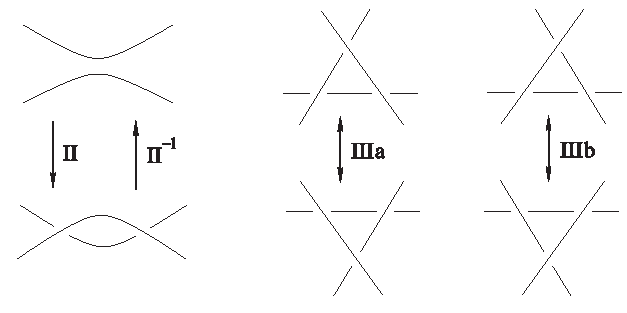
\includegraphics[width=.6\textwidth]{figs/reid_moves.pdf}
\caption{Legendrian Reidemeister Moves}
\label{fig:reid_moves}
\end{figure}

Note that the third Reidemeister move has two version, both preserving the number
of crossings, whereas the second does not. 
\comment{( The first Reidemeier move can not be realized as a Legendrian
isotopy, because it does not preserve the rotation number. )} 
We will see that for in either of the two versions of the third move the \Ainf-algebra changes by a tame isomorphism. 
In the case of the second move we will also need to stabilize, since
the number of crossings has changed.

\newcommand{\Ypm}{Y_{t'\pm\epsilon}}
\newcommand{\Yp}{Y_{t'\pm\epsilon}}
\newcommand{\Ym}{Y_{t'\pm\epsilon}}

Suppose a bifurcation occurs at $t = t'$. Consider a small $\epsilon > 0$ and let
$(A^\pm, m^\pm) = (A_{L_{t\pm\epsilon}}, m_{L_{t\pm\epsilon}})$. 
Without loss of generality, we will assume that for $t\in[t'-\epsilon, t'+\epsilon]$ the projection of the knot is unchanged
outside a small neighbourhood of where the bifurcation occurs. 


 %% TODO
    
\subsection{Move IIIa}
Let $A^\pm = A = \Z_2\<{a,b,c, a_1, ..., a_l}$ where $a,b$ and $c$ are as shown in
figure \pref{fig:move_iiia} and $a_1,...,a_l$ denote the crossing outside a
neighbourhood of the bifurcation. Note that the grading of $a,b$ and $c$
are the same in both diagrams and thus $A^+$ and $A^-$ are isomorphic as graded
vector spaces. We claim that $m^+ = m^-$. 
To prove this we will, by continuity, construct a bijective map
$R_k: W^+_k(\Ym) \to W^+_k(\Yp)$
such that for each $f \in W^+_k(\Ym)$ and vertex $x_i^k$ of $\Pi_k$, 
\[ R(f)(x_i^k) = f(x_i^k) \in \Z_2\<{a,b,c, a_1, ..., a_l}. \]
It then follows immediately that $m^+ = m^-$.

\begin{figure}
\centering
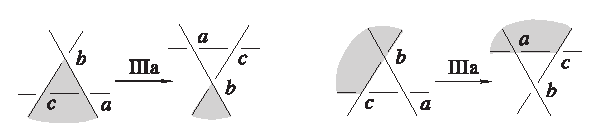
\includegraphics[width=.6\textwidth]{figs/move_iiia.pdf}
\caption{}
\label{fig:move_iiia}
\end{figure}

Let $f^\pm \in W^+_3(\Ypm)$ be the immersions whose image is
the small triangles with vertices $a,b,c$ and let $R(f_-)=f_+$. Then by Corollary
\pref{prop:height_sum}, 

\begin{equation}
\label{eq:habc}
H(a) > H(b) + H(c), 
\end{equation}

\begin{lemma}
\label{prop:habc}
Let $f\in W_k^+(\Ypm)\setminus\{f_\pm\}$, then neither of the
segments $[a,b], [b,c], [a,c]$ is the image of an edge of $\Pi_k$ under the
immersion $f$.
\end{lemma}

\begin{proof}
If $[a,b]$ (resp. $[a,c]$) is the image of an edge of $\Pi_k$, the vertex sent
$b$ (resp.  $c$) is positive and that sent to $a$ negative. Then
Corollary \ref{prop:height_sum} would imply $H(b) > H(a)$ (resp. $H(a) > H(c)$),
which would contradict \pref{eq:habc}. If $[b,c]$ is the image of an edge, both
$b$ and $c$ would be positive and thus $f$ would not be admissible.
\end{proof}

Assume $f \in W_k^+(\Ym)\setminus\{f_-\}$ such that one of the
vertices is mapped to $a,b$ or $c$. Then, by lemma \ref{prop:habc}, $f$ can be
deformed, continuously in $t$, to an immersion $R(f) \in W_k^+(\Yp)$
as shown in figure \ref{fig:move_iiia}. 

By changing the direction of time, the very same construction defines a map 
$R': W_k^+(\Yp) \to W_k^+(\Ym)$ which is inverse to $R$.

    
\subsection{Move IIIb}
Let $A^\pm = A = \Z_2\<{a,b,c, a_1, ..., a_l}$ where $a,b$ and $c$ are as shown in
figure \ref{fig:move_iiib} and again $a_1,...,a_l$ denote the crossing outside a
neighbourhood of where the bifurcation occur. Again, the grading of
$a,b$ and $c$ is unchanged and thus $A^+$ and $A^-$ are isomorphic as graded
vector spaces.

\figpdf{.6}{move_iiib}{.}

Let $f_\pm \in \tilde{W}_3(Y)$ be the immersion whose images are the small
triangles $T_\pm$ with vertices $a,b,c$, then by lemma
\pref{prop:deg_sum}, we find that $\deg(a) = \deg(bc)$.

Let $g: TA \to A$, such that $g_2(b,c) = a$, $g_1 = \id_A$
and $g$ is otherwise zero. Then $g^2 = g \circ g = \id^A$, since 
\[ g^2(b,c) = g_2(g_1(b),g_1(c)) + g_1(g_2(b,c)) = a+a = 0, \]
and we claim, 
\begin{equation}
\label{eq:move_iii_a_inf_rel}
\sum_{r,s,t} g_u(\I^{\otimes r} \otimes m^+_s \otimes \I^{\otimes t}) 
= m^-_n \circ g 
% \quad \qty( := \sum_{i_1,...i_r} m^-_r (g_{i_1} \otimes g_{i_2} \otimes ... \otimes g_{i_r}) ) .
\end{equation}
So $g$ is a tame \Ainf-isomorphism from $(A, m^+)$ to $(A,m^-)$.

\begin{remark}
In addition to \pref{eq:move_iii_a_inf_rel}, we also requite that the equation
with plus and minus swapped is satisfied. Since this is the condition for $g =
g^{-1}: (A, m^+) \to (A,m^-)$, to be an \Ainf-homomorphism. 
However, this follows immediately, by the symmetry of the problem when
reversing the direction of time.
\end{remark}

\lskip
Consider $f \in W^+_k(Y_{t'\pm \epsilon})$, then the triangle $T_\pm$ cannot be
the image of $f$, since it a two positive vertices. Assume $f$ maps an edge
$X_i$ of $\Pi_k$ to one of the sides of $T_\pm$. Then a
neighbourhood of $X_i$ is mapped to one of the shaded areas in
\pref{fig:move_iiib}. If the shaded area is marked with (1) or (2), clearly $f
\in W^+_k(\Ypm,a)$ (ie. $f(x^k_0) = a$,) since $a$ is positive. 

\begin{lemma}
If the shaded area marked by (3), $f(x^k_0) = a_i$ for some $i \in
\{1,...,l\}$.
\end{lemma}

\begin{proof}
Indeed, by corollary \pref{prop:height_sum}, $f(x^k_0) \ne
f(x^k_i)$ for $i\ne0$, so $f(x^k_0)$ cannot be $b$ nor $c$. 
Also if $f(x^k_0) = a$, then by lemma \pref{prop:l_6.1}, 
\[ H(a) - H(b) - H(c) > |f(\Pi_k)| > 0. \]
However, by applying lemma \pref{prop:l_6.1} to the $f_\pm$, 
$H(b) + H(c) - H(a) = |T_\pm| > 0$.
\end{proof}

In order to prove the claim \pref{eq:move_iii_a_inf_rel} we will simplify
the problem, by fixing a generator $v \in \Cc$ and consider the problem
restricted to the one-dimensional subspace spanned by $v$. ie. 
\begin{equation}
\label{eq:move_iii_a_inf_rel_pr}
\pr_v \circ \left\{ \sum_{r,s,t} g_u(\I^{\otimes r} \otimes m^+_s \otimes \I^{\otimes t})
\right\} = \pr_v \circ\:  m^-_n \circ g . 
%
%= \pr_v \left\{ \sum_{i_1,...,i_r} m^-_r (g_{i_1} \otimes g_{i_2} \otimes ... \otimes g_{i_r}) \right\}.  
\end{equation}



\subsubsection{Case $v \ne a$:}
First, we'll assume $v \ne a$. Then by the definition of $g_n$, 
$\pr_v \circ \: g_n = 0$ if $n\ne 1$ and $g_1 = \id_A$, so the left hand side of the equation
simplifies to $\pr_v \circ\: m^+_n$. 

To prove this equation, there are 6 different kinds of fragments, we
need to consider (Numbered $a_\pm, b_\pm$ and $c_\pm$ in figure
\pref{fig:move_iiib1} ).

\figpdf{.8}{move_iiib1}{.}

\newcommand{\tA}{\tilde{A}}
\newcommand{\tC}{\tilde{\Cc}}
\newcommand{\tm}{\tilde{m}}

It turns out that the terms in $m^\pm$ coming from fragments that look like
$a_\pm$ transforms differently form terms coming from $b_\pm$. In order to
distinguish between these two cases we will define a new vectors space
$\tA = \Z_2\<{a',a'',b,c,a_1,...,a_l}$ and a family of maps
\[ \tm^\pm_k : \tA^{\otimes k} \to \tA.  \]
(Note that we will not require that the maps satisfy the \Ainf relations.)
Let $\tC = \{ a',a'',b,c,a_1,...,a_l\}$ denote the set of generators.

Like in section \pref{sect:Ainf_m}, let $v_1,...,v_k \in \tC$ and 
\[ \tilde{\M}^v_{v_1,...,v_k}(Y_{t'\pm\epsilon}) = \{ u \in W^+_k (Y_{t'\pm\epsilon},v) \q| u(x^k_i) = v_i \}, \]
where by $u(x^k_i) = a'$ (resp. $u(x^k_i) = a''$), we means that $u(x^k_i) = a$
and a neighbourhood of $x^k_i$ in $\Pi_k$ is mapped to the shaded area in
\pref{fig:move_iiib1}, marked by $a_\pm$ (resp. $b_\pm$). For $v_1,...,v_k \in \tC$, define 
\[ \tm^\pm_k(v_1,...,v_k) = \sum_{v\in\tC} (\#_2
\tilde{\M}^v_{v_1,...,v_k}(Y_{t'\pm\epsilon})) v. \]

Define $\sigma : TA \to \tA$, by $\sigma_1(v) = v$ for all 
$v\in \{ b,c,a_1,...,a_n \}$, \[  \sigma_1(a) = a' + a'' \] and $\sigma_k = 0$ for
$k>1$. Also define $g', g'': T\tA \to \tA$, by 
\[ g'_1 = g''_1 = \id_{\tA}, \quad g'_2(b,c) = a', \quad g''_2(b,c) = a''  \]
and both are otherwise 0. Since $(\tA,m^\pm)$, is not an \Ainf-algebra,
it make non sense to speak of these maps as \Ainf-homomorphisms. However we
can still, consider their composition like definition \pref{def:Ainf_comp}.
Then it is quite easy to check that 
\begin{equation}
\label{eq:sigma_g}
\sigma \circ g = g' \circ g'' \circ \sigma 
\qq\tand
\pr_v \circ\: m^- = \pr_v \circ\: \tm^m \circ\: \sigma. 
\end{equation}

\newcommand{\bm}{\overline{m}}

We will define two  more families of maps $\bm_k: A^{\otimes k} \to A$. 
Consider the subset $S_\pm(v) \subset W^+(Y_\pm,v)$ 
( her $W^+(\Ypm) = \bigcup_{k\ge 1} W^+_k(\Ypm,v)$, ) consisting of immersions, which contain no fragment 
%(ie. image of a neighbourhood of an edge of $\Pi_n$)
marked by $c_\pm$ in \pref{fig:move_iiib1}. For $v_1,...,v_k \in \tC$, define 
%
\begin{equation}
\bm^\pm_k(v_1,...,v_k) = \sum_{v\in \tC } \qty(\#_2\qty(
\tilde{\M}^v_{v_1,...,v_k}(Y_{t'\pm\epsilon}) \cap S^{\pm}(v) )) v. 
\end{equation}

% \begin{align*}
% \bm^\pm_k(v_1,...,v_k) &= \sum_{v\in \tC } (\#_2
% \overline{\M}^v_{v_1,...,v_k}(Y_{t'\pm\epsilon}))v, \\ \q{\text{where}} 
% %
% \overline{\M}^v_{v_1,...,v_k} (Y_{t'\pm\epsilon}) 
% &= \tilde{\M}^v_{v_1,...,v_k}(Y_{t'\pm\epsilon}) \cap S^\pm(v).
% \end{align*}

% Denote $\theta_\pm = \{ (u(x^n_1),...,u(x^n_n)) \q| u \in S_\pm \} \subset
% A^{n}$ (ie. Topples, $(v_1,...,v_n)$, such that $m^{\pm}(v_1,...,v_n) = v$,
% and which does not contain $...,b,c,...$ ).

Like in the case of move iiia, all immersions $u\in S_-(v)$ deforms
continuously through $t=t'$, defining a bijection $S_-(v) \to S_+(v)$. See fig
\pref{fig:move_iiib2}. So, actually $\bm^+ = \bm^-$.

\figpdf{.6}{move_iiib2}{}

Let $u \in S_+(v)$ (resp. $u\in S_-(v)$) and let $M_u \subset \{1,...,k\}$, such that $u(x_i) = a$
and a neighbourhood of $x_i$ is mapped to the shaded
area marked by $a_+$ (resp. $b_-$) in fig. \pref{fig:move_iiib2}. (Note that might both no such
fragments, in which case $M_u$ is empty and there might be multiple 
fragments $\Pi_k$ this same area.)
Given $C \subset M_u$, define $u^C \in W^+_{n+|C|}(Y_+, v)$, by
replacing the fragment near $x_i$, for each $i \in C$, as shown in figure
\pref{fig:move_iiib3}. 

\begin{figure}[h]
\centering
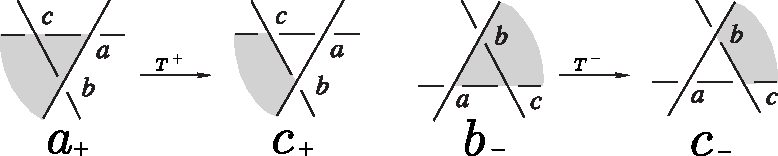
\includegraphics[width=.6\textwidth]{figs/move_iiib3.pdf}
\caption{}
\label{fig:move_iiib3}
\end{figure}

Define the map $T_u^+ : \mathcal{P}(M_u) \to \bigcup_{k\ge 1} W^+_k(\Ypm,v)$,
by  $C \mapsto u^C$. Then
\footnote{Here $\mathcal{P}(M_u)$ denotes the power set.}
\begin{equation}
\label{eq:sq_union_T}
W^+(\Ypm,v) = \bigsqcup_{u\in S^-(v)} T_u^{-} 
\end{equation}

We clime that this implies 
\begin{equation}
\label{eq:tm_as_bm_and_gm}
\pr_v \circ\: \tm^+ = \pr_v \circ\: \bm^+ \circ\: g' 
\qq\tand \pr_v \circ\: \tm^- = \pr_v \circ\: \bm^- \circ\: g''. 
\end{equation}

Let $(v_1,...,v_k) \in A^{\otimes k}$, write 
\[ (v_1,...,v_k) = (v_{I_1}, b, c, v_{I_2}, ..., b,c, v_{I_p}), \]
where $v_{I_1} \in A^{\otimes I_1}$ is a tuple containing no
consecutive $b,c$. Then if there exists $u' \in W^+_{k+1}(\Ypm,v)$, 
such that $(v_1,...,v_k) = (u'(x^k_1), ..., u'(x^{k+1}_{k}))$. By 
eq. \pref{eq:sq_union_T}, $u' = T_u^+(C)$ for some $\in S_+(v)$ and $C \in \{
1,...,k\}$. ( Actually, we most have $C = (I_1+1, I_2+2, ..., v_{I_p} + p)$ ). So 
\[ (v_{I_1}, g'(b,c),v_{I_2},...,g'(b,c),v_{I_p}) =
\qty(u(x^{k-|C|}_1),...,u(x^{k-|C|}_1)). \]
Hence for every term in $\tm^+(v_1,...,v_k)$ there is a corresponding term in
$(\bm^+ \circ g')(v_1,...,v_k)$. It is easy to check that also the converse
hold and the argument for the second equation is exactly the same.

Finally, by combining the above relations, \pref{eq:sigma_g},
\pref{eq:tm_as_bm_and_gm} and $\bm^+ = \bm^-$, as well as the fact that
$(g')^2 = \id$, we have 
%
\begin{align*}
m^- \circ g 
&= \tm^- \circ\: \sigma \circ\: g \\
&= \tm^- \circ\: g'' \circ\: g' \circ\: \sigma \\
&= \bm^- \circ\: g' \circ \sigma  \\
&= \bm^+ \circ\: g' \circ \sigma  \\
&= \tm^+ \circ \sigma   \\
&= m^+.
\end{align*}
(Note, we have suppressed the $\pr_v$ at the beginning of each line in the above
calculations. The equalities only hold in the subspace spanned by $v\ne a$.)


\subsubsection{Case $v = a$:}
When $v = a$, $g$ does no longer disepere from the LHS of equation
\pref{eq:move_iii_a_inf_rel_pr}, though, by the simplisity of $g$, it does simplify
%
\begin{align*}
LHS &:= \pr_v \circ\: \qty{ \sum_{r,s,t} g_u(\I^{\otimes r} \otimes m^+_s
\otimes \I^{\otimes t}) } \\
&= g_1 (\pr_a \circ\: m^+_n) + g_2(\pr_b, \pr_c \circ\: m^+_{n-1})
+ g_2(\pr_b \circ\: m^+_{n-1}, \pr_c).
\end{align*}

By Lemma \pref{prop:l_6.1}, we can, by decreasing $\epsilon$ if necessary,
that $H(a) > H(b), H(c)$. Hence by corollary
\pref{prop:height_sum}, 
\[ \pr_v \circ\: m^+(...,a,...) = 0, \quad\text{for } v = a,b,c. \]
Therefore the RHS of equation \pref{eq:move_iii_a_inf_rel_v}, simplifies
\[ RHS := \pr_a \circ\: m^-_n \circ\: g = \pr_a \circ\: m^-_n. \]

There are only two kinds of fragments that are relevant, the ones marked
by (1) and (2) in figure \pref{fig:move_iiib}. For $i=1,2$, let $S^{\pm,i}_k
\subset W^+_k(\Ypm, a)$ denote the set of immersions that maps a
neighbourhood of $x^k_0$ to the shaded area marked by (i). Like above we will
define pre-\Ainf-structures $\tm^{\pm, i}_n : A^{\otimes n} \to A$. 
Given $v_1,...,v_n \in \Cc$, define 
%
\begin{equation}
\tm^{\pm, i}_k(v_1, ..., v_k) = \sum_v \qty(\#_2\qty(
\tilde{\M}^v_{v_1,...,v_k}(\Ypm) \cap S^{\pm, i}_k))  v.
\end{equation}

    
\subsection{Move II}
Let $a,b$ be the two crossings in $\Ym$, which vanish during the
bifurcation. By slightly perturbing $L_t$ and decreasing $\epsilon$ if necessary,
we number the crossings of $\Ym$ by $a,b,a_1,...,a_l,b_1,...,b_m$ in such a way
that (through out the bifurcation. Ignoring $a,b$ after they have vanished)
\[ H(a_l) \ge ... \ge H(a_1) \ge H(a) > H(b) \ge H(b_1) \ge ... \ge
H(b_m). \]
Here, $H(a)$ denotes the absolute difference between the $z$-values of the two
parts of $L_t$, projection down to $a$.

Note that, by lemma \pref{prop:l_6.1}, the difference between $H(a)$ and $H(b)$
equals the area of the curved 2-gon (let's call it $D$), which vanish at $t=t'$.  
Let $\bar{f} \in W^+_2(Y,a)$ be the immersion whose image is $D$. Then,
since the area of $D$ and thus also the difference between $H(a)$ and
$H(b)$, corollary \pref{prop:height_sum} implies that, there cannot be any
immersion $u \in W^+_k(\Ym, a)$ mapping a vertex to $b$, except $\bar{f}$.
Therefore 
\[ \pr_a \circ\: m^-(...,b,...) = 0,\quad \text{(except if both the $...$'s are
empty)}. \]
Hence $\pr_a \circ\: m^- = \delta^a_b + a f$, where $\delta^a_b:
TA \to A$ and $f: TA \to \Z_2$, are given by
\[(\delta^a_b)_1(b) = a, \quad  (\delta^a_b)_1(v) = 0, \quad (\delta^a_b)_k = 0, \quad
\forall v \ne b, k \ge 1,\]
and 
\[ f(...,v,...) = 0, \quad \forall v \in \{ a,b,a_1,...,a_n \}. \]

Denote $(A,m) = (A^+, m^+)$, where $A=\Z_2\<{a_1,...,a_l,b_1,...,b_m}$ and
let $(A', m') = (S_i(A),m^{S_i(A)})$, where $i = |a|$. 
We want to show that $(A^-, m^-)$ and $(A, m')$ are tame-isomorphic. 

We'll start by defining the \Ainf-pre-homomorphism $s: A' \ato A^-$, given by 
$s = \tilde{s} + b f$, where $\tilde{s}: A' \ato A^-$ is the strict
\Ainf-homomorphism mapping $e_1, e_2$ to $a$ and $b$ respectively and fixes $a_i$ and $b_i$.

\newcommand{\hm}{\widehat{m}}

Let $\hm$ be the unique \Ainf-structure, from lemma 
\pref{lemma:Ainf_struct_from_pre_hom}, such that $s$ is an
\Ainf-homomorphism. Then by construction $(A^-, m^-)$ and $(A',
\hm)$ are tame isomorphic. 

Let $A_{[i]} = \Z_2\<{a_1,...,a_i, b_1,...,b_m, e_1,e_2}$, for each $i\in
\{0,...,l\}$ and let $\tau : A \ato A'$ be the inclusion, from
\pref{lemma:tau_id_homotopy}. Then

\begin{lemma}
\label{lemma:move_ii_alpha}
\begin{itemize}
\item[a)] $\pr_{[0]} \circ\: \hm  = \pr_{[0]} \circ\: m'$, where
$\pr_{[i]}$ is the projection onto $A_{[i]}$,
\item[b)] $m' \circ\:\tau = \hm \circ\: \tau$.
\end{itemize}
\end{lemma}

In order to show that $(A', \hm)$ is also
tame isomorphic to $(A', m')$, we will inductively construct a sequence of
tame isomorphic \Ainf-structures $(A', m^{[i]})$. Such that, $(A', m^{[0]}) =
(A', \hm)$, for each $i \in \{ 0,...,l \}$,
\[ \pr_{[i]} \circ\: m^{[i]}  = \pr_{[i]} \circ\: m'. \]
Note that, for $i=l$, $\pr_{[l]} = \id_{A'}$, and thus $(A',m') =
(A',m^{[l]})$, concluding the proof. Also note that the case of $i=0$ is satisfied,
by lemma \pref{lemma:move_ii_alpha}, which we will prove after
constructing the $m^{[i]}$'s. 

Suppose we have already defined $m^{[0]}, ..., m^{[j-1]}$. To define
$m^{[j]}$, we first define an \Ainf-pre-homomorphism $g^j: A' \ato A'$ 
(with $g^1$ an isomorphism) and define
$m^{[j]}$ to be the \Ainf-structure on $A'$, such that $g^j$ is an
\Ainf-homomorphism from $(A',m^{[j]})$ to $(A',m^{[j-1]})$.

Let $c^j, q^j : A' \ato A'$ be \Ainf-pre-homomorphisms, given by, 
\begin{equation}
\label{eq:c_q_def}
c^j = \pr_{a_j} \circ\: \qty{ m' + m^{[j-1]} } \qq\tand 
q^j = c^j \circ h,
\end{equation}
where $h: A' \ato A'$ is the \Ainf-homotopy, from lemma
\pref{lemma:tau_id_homotopy}. Then define $g^j := \id_{A'} + q^j$.

It follows immediately from the definition of $h$, that
\begin{equation}
\label{eq:q_j_simple}
q^j(...,a_k,...) = 0, \quad \forall k \ge j.
% \text{unless } v = e_1,
\end{equation}
Hence $g^j$ is tame and $g^j_1$ is an isomorphism. 

Since $g^j$ is an \Ainf-homomorphism, the following \Ainf-relations,
\begin{equation}
\label{eq:g_j_Ainf_rels}
\sum_{r,s,t} g^j_u (\I^{\otimes r} \otimes m^{[j]}_s \otimes 
\I^{\otimes t}) = (m^{[j-1]} \circ g^j)_n. 
\end{equation}
%
By projecting eq. \ref{eq:g_j_Ainf_rels} onto $A_{[j-1]}$, we have
\[ LHS = \pr_{[j-1]} \circ\: m^{[j]}_n, \quad \text{since } \pr_{[j-1]}
\circ\: q^j = 0. \]
And, using the inductive hypothesise,
\[ RHS = \pr_{[j-1]} \circ\: m'_n + \pr_{[j-1]} \circ\: ( m' \circ q^j )_n, \]
where the last term disappears, by corollary \pref{prop:height_sum}.

It remains to prove that $\pr_{a_j} \circ\: m^{[j]}_n = \pr_{a_j} \circ\:
m'_n$. Projecting eq. \ref{eq:g_j_Ainf_rels} onto $a_{j}$, we have
\[  LHS = \pr_{a_j} \circ\: m^{[j]}_n + \sum_{r,s,t} q^j_u
(\I^{\otimes r} \otimes m^{[j]}_s \otimes \I^{\otimes r}), \]
By eq. \ref{eq:q_j_simple} and since 
$\pr_{[j-1]} \circ\: m^{[j]}_s = \pr_{[j-1]} \circ\: m'_s$, 
\[ q^j_u(\I^{\otimes r} \otimes m^{[j]}_s \otimes \I^{\otimes r})
 = q^j_u(\I^{\otimes r} \otimes m'_s \otimes \I^{\otimes r})
\]
And $RHS = \pr_{a_j} \circ\: (m^{[j-1]} \circ\: g^j)_n$. 

\begin{lemma}
\label{lemma:move_ii_beta}
For all $k \ge j$ and $n$, 
\[ (\pr_{a_j} \circ\: m^{[j-1]})_n(...,a_k,...) = 0. \]
\end{lemma}

\begin{proof}
By lemma 6.1, the claim holds for $j=1$. We show that the equation holds any
$j$ by induction on $j$ and $n$. Suppose the equation holds for $j-1$. Then,
by the explicit construction of $m^{[j]}$, in the proof of lemma
\pref{lemma:Ainf_struct_from_pre_hom}, 
\[  m^{[j]}_n = \sum_{r,s<n,t} g^j_u (\I^{\otimes r} \otimes m^{[j]}_s \otimes
\I^{\otimes t}) + ( m^{[j-1]}_r \circ\: g^j )_n. \]
Applying the RHS on $(..., a_k, ...)$ (and projection onto $a_j$), the $g^j$ in the last term acts
as the identity, by equation \ref{eq:q_j_simple}, and thus the last term vanish
by the inductive hypothesise. When $n=1$, there is no first term (Note that we are ignoring the curvature, ie. $n=0$, since we are
applying it to at least $a_k$.), so this case is immediate. It then also
follows, by simple induction on $n$, that the RHS, vanish for all $n$. 
\end{proof}

By corollary \pref{prop:height_sum}, $\pr_{a_j} \circ\: m'(...,a_k,...) = 0$. 
Therefore it follows from lemma \pref{lemma:move_ii_beta} that also
\begin{equation}
\label{eq:c_on_a_k_vanish}
\pr_{a_j} \circ\: c^j(...,a_k,...) = 0. 
\end{equation}

By lemma \pref{lemma:move_ii_beta}, the $g$ on the RHS acts as the
identity, so we have (suppressing the $\pr_{a_j}$ at the beginning of each
line)
\begin{align*}
m^{[j]}_n 
&= m^{[j-1]}_n + \sum_{r,s,t} q^j_u (\I^{\otimes r} \otimes m^{[j-1]}_n\otimes
\I^{\otimes t}) \\
&= m'_n + c^j_n + \sum_{r,s,t} ( c^j \circ\: h )_u(\I^{\otimes r} \otimes m^{[j-1]}_n\otimes
\I^{\otimes t}), & \text{by eq. } \ref{eq:c_q_def} \\
&= m'_n + c^j_n + \sum_{r,s,t} c^j (h_1\otimes ... \otimes h_1)(\I^{\otimes r}
\otimes m^{[j-1]}_n\otimes \I^{\otimes t}) \\
&= m'_n + c^j_n + 
\end{align*}




